\documentclass[]{article}
\usepackage{lmodern}
\usepackage{amssymb,amsmath}
\usepackage{ifxetex,ifluatex}
\usepackage{fixltx2e} % provides \textsubscript
\ifnum 0\ifxetex 1\fi\ifluatex 1\fi=0 % if pdftex
  \usepackage[T1]{fontenc}
  \usepackage[utf8]{inputenc}
\else % if luatex or xelatex
  \ifxetex
    \usepackage{mathspec}
  \else
    \usepackage{fontspec}
  \fi
  \defaultfontfeatures{Ligatures=TeX,Scale=MatchLowercase}
\fi
% use upquote if available, for straight quotes in verbatim environments
\IfFileExists{upquote.sty}{\usepackage{upquote}}{}
% use microtype if available
\IfFileExists{microtype.sty}{%
\usepackage{microtype}
\UseMicrotypeSet[protrusion]{basicmath} % disable protrusion for tt fonts
}{}
\usepackage[margin=1in]{geometry}
\usepackage{hyperref}
\hypersetup{unicode=true,
            pdftitle={Expenses},
            pdfauthor={Axel-Cleris Gailloty},
            pdfborder={0 0 0},
            breaklinks=true}
\urlstyle{same}  % don't use monospace font for urls
\usepackage{color}
\usepackage{fancyvrb}
\newcommand{\VerbBar}{|}
\newcommand{\VERB}{\Verb[commandchars=\\\{\}]}
\DefineVerbatimEnvironment{Highlighting}{Verbatim}{commandchars=\\\{\}}
% Add ',fontsize=\small' for more characters per line
\usepackage{framed}
\definecolor{shadecolor}{RGB}{248,248,248}
\newenvironment{Shaded}{\begin{snugshade}}{\end{snugshade}}
\newcommand{\AlertTok}[1]{\textcolor[rgb]{0.94,0.16,0.16}{#1}}
\newcommand{\AnnotationTok}[1]{\textcolor[rgb]{0.56,0.35,0.01}{\textbf{\textit{#1}}}}
\newcommand{\AttributeTok}[1]{\textcolor[rgb]{0.77,0.63,0.00}{#1}}
\newcommand{\BaseNTok}[1]{\textcolor[rgb]{0.00,0.00,0.81}{#1}}
\newcommand{\BuiltInTok}[1]{#1}
\newcommand{\CharTok}[1]{\textcolor[rgb]{0.31,0.60,0.02}{#1}}
\newcommand{\CommentTok}[1]{\textcolor[rgb]{0.56,0.35,0.01}{\textit{#1}}}
\newcommand{\CommentVarTok}[1]{\textcolor[rgb]{0.56,0.35,0.01}{\textbf{\textit{#1}}}}
\newcommand{\ConstantTok}[1]{\textcolor[rgb]{0.00,0.00,0.00}{#1}}
\newcommand{\ControlFlowTok}[1]{\textcolor[rgb]{0.13,0.29,0.53}{\textbf{#1}}}
\newcommand{\DataTypeTok}[1]{\textcolor[rgb]{0.13,0.29,0.53}{#1}}
\newcommand{\DecValTok}[1]{\textcolor[rgb]{0.00,0.00,0.81}{#1}}
\newcommand{\DocumentationTok}[1]{\textcolor[rgb]{0.56,0.35,0.01}{\textbf{\textit{#1}}}}
\newcommand{\ErrorTok}[1]{\textcolor[rgb]{0.64,0.00,0.00}{\textbf{#1}}}
\newcommand{\ExtensionTok}[1]{#1}
\newcommand{\FloatTok}[1]{\textcolor[rgb]{0.00,0.00,0.81}{#1}}
\newcommand{\FunctionTok}[1]{\textcolor[rgb]{0.00,0.00,0.00}{#1}}
\newcommand{\ImportTok}[1]{#1}
\newcommand{\InformationTok}[1]{\textcolor[rgb]{0.56,0.35,0.01}{\textbf{\textit{#1}}}}
\newcommand{\KeywordTok}[1]{\textcolor[rgb]{0.13,0.29,0.53}{\textbf{#1}}}
\newcommand{\NormalTok}[1]{#1}
\newcommand{\OperatorTok}[1]{\textcolor[rgb]{0.81,0.36,0.00}{\textbf{#1}}}
\newcommand{\OtherTok}[1]{\textcolor[rgb]{0.56,0.35,0.01}{#1}}
\newcommand{\PreprocessorTok}[1]{\textcolor[rgb]{0.56,0.35,0.01}{\textit{#1}}}
\newcommand{\RegionMarkerTok}[1]{#1}
\newcommand{\SpecialCharTok}[1]{\textcolor[rgb]{0.00,0.00,0.00}{#1}}
\newcommand{\SpecialStringTok}[1]{\textcolor[rgb]{0.31,0.60,0.02}{#1}}
\newcommand{\StringTok}[1]{\textcolor[rgb]{0.31,0.60,0.02}{#1}}
\newcommand{\VariableTok}[1]{\textcolor[rgb]{0.00,0.00,0.00}{#1}}
\newcommand{\VerbatimStringTok}[1]{\textcolor[rgb]{0.31,0.60,0.02}{#1}}
\newcommand{\WarningTok}[1]{\textcolor[rgb]{0.56,0.35,0.01}{\textbf{\textit{#1}}}}
\usepackage{graphicx,grffile}
\makeatletter
\def\maxwidth{\ifdim\Gin@nat@width>\linewidth\linewidth\else\Gin@nat@width\fi}
\def\maxheight{\ifdim\Gin@nat@height>\textheight\textheight\else\Gin@nat@height\fi}
\makeatother
% Scale images if necessary, so that they will not overflow the page
% margins by default, and it is still possible to overwrite the defaults
% using explicit options in \includegraphics[width, height, ...]{}
\setkeys{Gin}{width=\maxwidth,height=\maxheight,keepaspectratio}
\IfFileExists{parskip.sty}{%
\usepackage{parskip}
}{% else
\setlength{\parindent}{0pt}
\setlength{\parskip}{6pt plus 2pt minus 1pt}
}
\setlength{\emergencystretch}{3em}  % prevent overfull lines
\providecommand{\tightlist}{%
  \setlength{\itemsep}{0pt}\setlength{\parskip}{0pt}}
\setcounter{secnumdepth}{0}
% Redefines (sub)paragraphs to behave more like sections
\ifx\paragraph\undefined\else
\let\oldparagraph\paragraph
\renewcommand{\paragraph}[1]{\oldparagraph{#1}\mbox{}}
\fi
\ifx\subparagraph\undefined\else
\let\oldsubparagraph\subparagraph
\renewcommand{\subparagraph}[1]{\oldsubparagraph{#1}\mbox{}}
\fi

%%% Use protect on footnotes to avoid problems with footnotes in titles
\let\rmarkdownfootnote\footnote%
\def\footnote{\protect\rmarkdownfootnote}

%%% Change title format to be more compact
\usepackage{titling}

% Create subtitle command for use in maketitle
\newcommand{\subtitle}[1]{
  \posttitle{
    \begin{center}\large#1\end{center}
    }
}

\setlength{\droptitle}{-2em}

  \title{Expenses}
    \pretitle{\vspace{\droptitle}\centering\huge}
  \posttitle{\par}
    \author{Axel-Cleris Gailloty}
    \preauthor{\centering\large\emph}
  \postauthor{\par}
      \predate{\centering\large\emph}
  \postdate{\par}
    \date{26/05/2019}


\begin{document}
\maketitle

\begin{Shaded}
\begin{Highlighting}[]
\CommentTok{# Load the packages }
\KeywordTok{library}\NormalTok{(tidyverse)}
\KeywordTok{library}\NormalTok{(FactoMineR)}
\KeywordTok{library}\NormalTok{(factoextra)}
\KeywordTok{library}\NormalTok{(highcharter)}
\KeywordTok{library}\NormalTok{(ggthemes)}
\KeywordTok{library}\NormalTok{(lubridate)}
\KeywordTok{library}\NormalTok{(treemap)}
\end{Highlighting}
\end{Shaded}

This kernel is under construction :) !

\hypertarget{reading-and-preparing-the-data}{%
\section{Reading and preparing the
data}\label{reading-and-preparing-the-data}}

\begin{Shaded}
\begin{Highlighting}[]
\NormalTok{fifa <-}\StringTok{ }\KeywordTok{read_csv}\NormalTok{(}\StringTok{"data.csv"}\NormalTok{)}
\KeywordTok{print}\NormalTok{(}\KeywordTok{paste}\NormalTok{(}\StringTok{"The dataset contains"}\NormalTok{, }\KeywordTok{dim}\NormalTok{(fifa)[}\DecValTok{1}\NormalTok{], }\StringTok{"observations and"}\NormalTok{, }\KeywordTok{dim}\NormalTok{(fifa)[}\DecValTok{2}\NormalTok{], }\StringTok{"columns"}\NormalTok{))}
\end{Highlighting}
\end{Shaded}

\begin{verbatim}
## [1] "The dataset contains 18207 observations and 89 columns"
\end{verbatim}

\hypertarget{missing-values}{%
\subsection{Missing values}\label{missing-values}}

With this said let's check the consistency of the dataset by looking for
missing values and understanding what each column stands for.

\begin{Shaded}
\begin{Highlighting}[]
\KeywordTok{theme_set}\NormalTok{(}\KeywordTok{theme_economist}\NormalTok{())}
\KeywordTok{map_dbl}\NormalTok{(fifa, }\ControlFlowTok{function}\NormalTok{(x) }\KeywordTok{sum}\NormalTok{(}\KeywordTok{is.na}\NormalTok{(x))}\OperatorTok{/}\KeywordTok{length}\NormalTok{(x)}\OperatorTok{*}\DecValTok{100}\NormalTok{) }\OperatorTok
\StringTok{  }\KeywordTok{stack}\NormalTok{() }\OperatorTok
\StringTok{  }\KeywordTok{ggplot}\NormalTok{(}\KeywordTok{aes}\NormalTok{(}\DataTypeTok{x =} \KeywordTok{reorder}\NormalTok{(ind,values), }\DataTypeTok{y =}\NormalTok{ values)) }\OperatorTok{+}\StringTok{ }
\StringTok{  }\KeywordTok{geom_bar}\NormalTok{(}\DataTypeTok{stat =} \StringTok{'identity'}\NormalTok{) }\OperatorTok{+}\StringTok{ }\KeywordTok{coord_flip}\NormalTok{() }\OperatorTok{+}
\StringTok{  }\KeywordTok{labs}\NormalTok{(}\DataTypeTok{y =} \StringTok{"% of missing values"}\NormalTok{, }\DataTypeTok{x =} \StringTok{"Columns"}\NormalTok{, }\DataTypeTok{title =} \StringTok{"Missing values"}\NormalTok{)}
\end{Highlighting}
\end{Shaded}

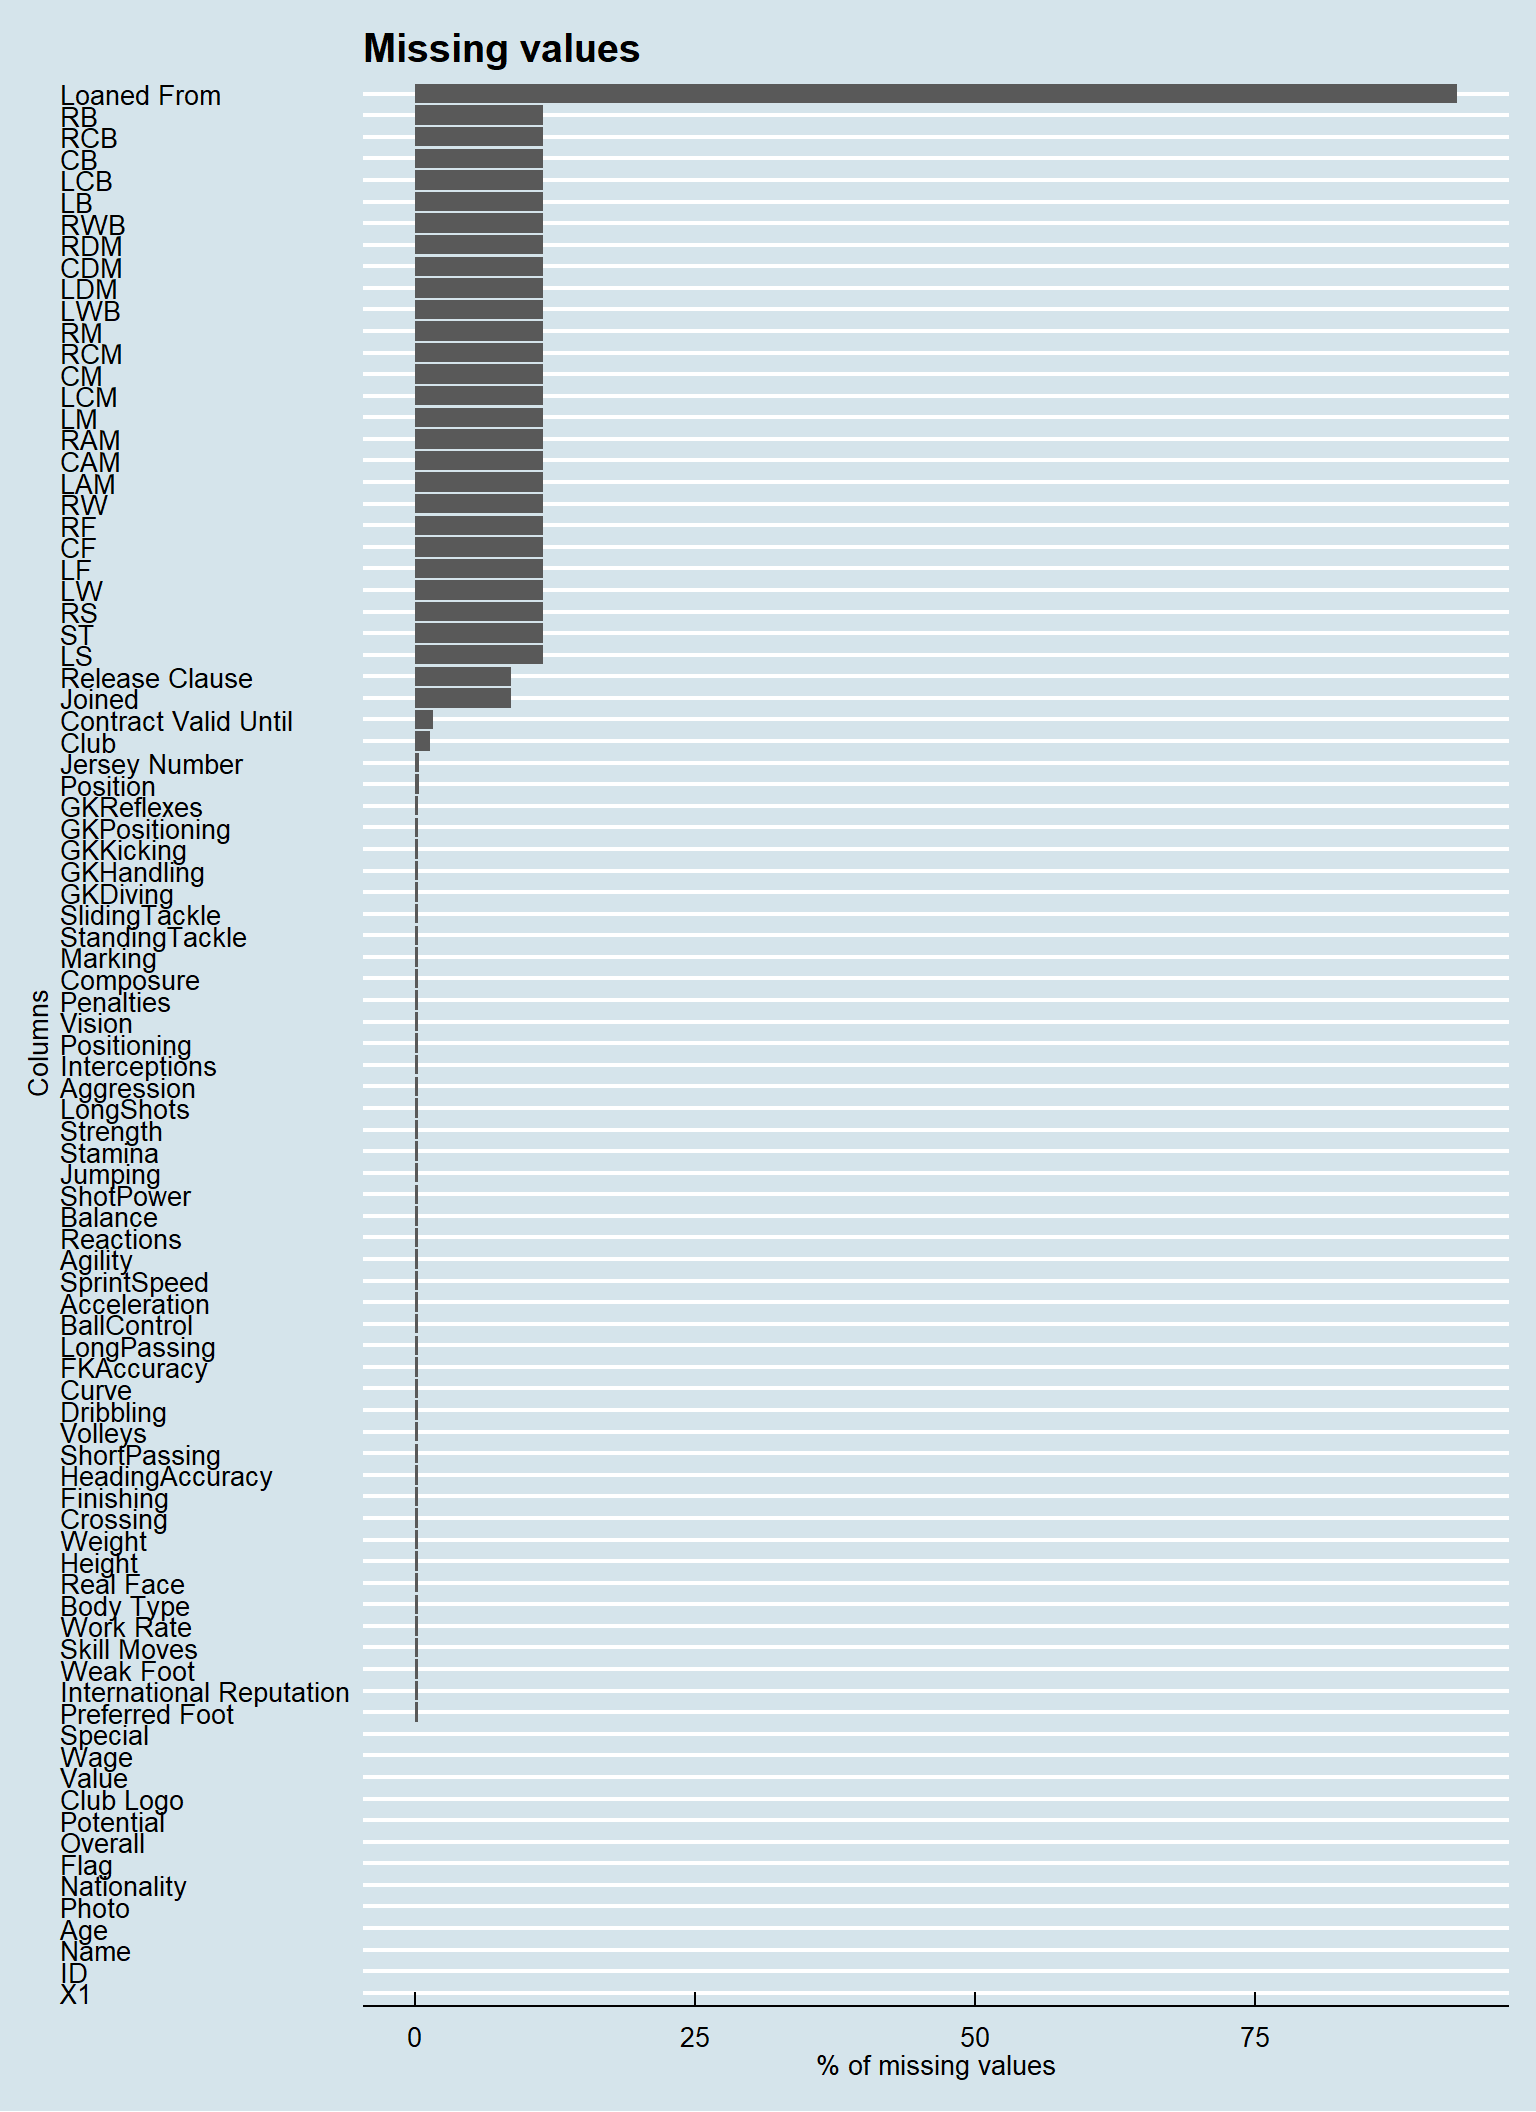
\includegraphics{football-cluster_files/figure-latex/unnamed-chunk-3-1.pdf}

The loaned from column contains lots of missing values. All the other
columns have between 0 and 10\% missing values. Overall the dataset
contains few missing values.

\hypertarget{columns-content}{%
\subsection{Columns content}\label{columns-content}}

\begin{Shaded}
\begin{Highlighting}[]
\KeywordTok{head}\NormalTok{(fifa)}
\end{Highlighting}
\end{Shaded}

\begin{verbatim}
## # A tibble: 6 x 89
##      X1     ID Name    Age Photo Nationality Flag  Overall Potential Club 
##   <dbl>  <dbl> <chr> <dbl> <chr> <chr>       <chr>   <dbl>     <dbl> <chr>
## 1     0 158023 L. M~    31 http~ Argentina   http~      94        94 FC B~
## 2     1  20801 Cris~    33 http~ Portugal    http~      94        94 Juve~
## 3     2 190871 Neym~    26 http~ Brazil      http~      92        93 Pari~
## 4     3 193080 De G~    27 http~ Spain       http~      91        93 Manc~
## 5     4 192985 K. D~    27 http~ Belgium     http~      91        92 Manc~
## 6     5 183277 E. H~    27 http~ Belgium     http~      91        91 Chel~
## # ... with 79 more variables: `Club Logo` <chr>, Value <chr>, Wage <chr>,
## #   Special <dbl>, `Preferred Foot` <chr>, `International
## #   Reputation` <dbl>, `Weak Foot` <dbl>, `Skill Moves` <dbl>, `Work
## #   Rate` <chr>, `Body Type` <chr>, `Real Face` <chr>, Position <chr>,
## #   `Jersey Number` <dbl>, Joined <chr>, `Loaned From` <chr>, `Contract
## #   Valid Until` <chr>, Height <chr>, Weight <chr>, LS <chr>, ST <chr>,
## #   RS <chr>, LW <chr>, LF <chr>, CF <chr>, RF <chr>, RW <chr>, LAM <chr>,
## #   CAM <chr>, RAM <chr>, LM <chr>, LCM <chr>, CM <chr>, RCM <chr>,
## #   RM <chr>, LWB <chr>, LDM <chr>, CDM <chr>, RDM <chr>, RWB <chr>,
## #   LB <chr>, LCB <chr>, CB <chr>, RCB <chr>, RB <chr>, Crossing <dbl>,
## #   Finishing <dbl>, HeadingAccuracy <dbl>, ShortPassing <dbl>,
## #   Volleys <dbl>, Dribbling <dbl>, Curve <dbl>, FKAccuracy <dbl>,
## #   LongPassing <dbl>, BallControl <dbl>, Acceleration <dbl>,
## #   SprintSpeed <dbl>, Agility <dbl>, Reactions <dbl>, Balance <dbl>,
## #   ShotPower <dbl>, Jumping <dbl>, Stamina <dbl>, Strength <dbl>,
## #   LongShots <dbl>, Aggression <dbl>, Interceptions <dbl>,
## #   Positioning <dbl>, Vision <dbl>, Penalties <dbl>, Composure <dbl>,
## #   Marking <dbl>, StandingTackle <dbl>, SlidingTackle <dbl>,
## #   GKDiving <dbl>, GKHandling <dbl>, GKKicking <dbl>,
## #   GKPositioning <dbl>, GKReflexes <dbl>, `Release Clause` <chr>
\end{verbatim}

\hypertarget{value-and-wage-columns}{%
\subsubsection{Value and wage columns}\label{value-and-wage-columns}}

\begin{Shaded}
\begin{Highlighting}[]
\KeywordTok{glimpse}\NormalTok{(fifa[}\KeywordTok{c}\NormalTok{(}\StringTok{"Value"}\NormalTok{, }\StringTok{"Wage"}\NormalTok{)])}
\end{Highlighting}
\end{Shaded}

\begin{verbatim}
## Observations: 18,207
## Variables: 2
## $ Value <chr> "€110.5M", "€77M", "€118.5M", "€72M", "€102M", "€93M", "...
## $ Wage  <chr> "€565K", "€405K", "€290K", "€260K", "€355K", "€340K", "€...
\end{verbatim}

Because of their formats \texttt{€-NUM-M/K}, R doesn't read them
properly. We need to do some string manipulations in order to convert
them into numerical columns so we can use later in the analysis.\\
Let's start by removing the \texttt{€}symbols in both columns.

\begin{Shaded}
\begin{Highlighting}[]
\NormalTok{fifa <-}\StringTok{ }\NormalTok{fifa }\OperatorTok\StringTok{ }\KeywordTok{mutate}\NormalTok{(}\DataTypeTok{Value =} \KeywordTok{str_replace}\NormalTok{(Value, }\StringTok{"€"}\NormalTok{, }\StringTok{""}\NormalTok{),}
                \DataTypeTok{Wage =} \KeywordTok{str_replace}\NormalTok{(Wage, }\StringTok{"€"}\NormalTok{, }\StringTok{""}\NormalTok{))}
\end{Highlighting}
\end{Shaded}

Now since since the \texttt{Value} column is not always in million € we
need to separate each element of it into two columns \texttt{raw\_value}
and \texttt{unit} that will hold the amount and the unit (millions (M)
or thousands(K))

\begin{Shaded}
\begin{Highlighting}[]
\NormalTok{fifa }\OperatorTok\StringTok{ }\KeywordTok{separate}\NormalTok{(Value, }\DataTypeTok{into =} \KeywordTok{c}\NormalTok{(}\StringTok{"raw_value"}\NormalTok{, }\StringTok{"unit_value"}\NormalTok{), }\DataTypeTok{sep =} \StringTok{"(?=[:LETTER:])"}\NormalTok{) }\OperatorTok
\StringTok{  }\KeywordTok{select}\NormalTok{(raw_value, unit_value) }\OperatorTok\StringTok{ }\KeywordTok{group_by}\NormalTok{(unit_value) }\OperatorTok\StringTok{ }\KeywordTok{summarize}\NormalTok{(}\DataTypeTok{count =} \KeywordTok{n}\NormalTok{())}
\end{Highlighting}
\end{Shaded}

\begin{verbatim}
## Warning: Expected 2 pieces. Missing pieces filled with `NA` in 252 rows
## [453, 539, 569, 678, 865, 875, 954, 998, 1009, 1121, 1272, 1353, 1603,
## 1672, 1820, 1903, 1908, 1934, 1937, 1965, ...].
\end{verbatim}

\begin{verbatim}
## # A tibble: 3 x 2
##   unit_value count
##   <chr>      <int>
## 1 K          11108
## 2 M           6847
## 3 <NA>         252
\end{verbatim}

As we can see here, there a fewer players who are worth million. Let's
save it and do the same for the Wage column.

\begin{Shaded}
\begin{Highlighting}[]
\NormalTok{fifa <-}\StringTok{ }\NormalTok{fifa }\OperatorTok\StringTok{ }\KeywordTok{separate}\NormalTok{(Value, }\DataTypeTok{into =} \KeywordTok{c}\NormalTok{(}\StringTok{"raw_value"}\NormalTok{, }\StringTok{"unit_value"}\NormalTok{), }\DataTypeTok{sep =} \StringTok{"(?=[:LETTER:])"}\NormalTok{)}
\end{Highlighting}
\end{Shaded}

\begin{Shaded}
\begin{Highlighting}[]
\NormalTok{fifa }\OperatorTok\StringTok{ }\KeywordTok{separate}\NormalTok{(Wage, }\DataTypeTok{into =} \KeywordTok{c}\NormalTok{(}\StringTok{"raw_wage"}\NormalTok{, }\StringTok{"unit_wage"}\NormalTok{), }\DataTypeTok{sep =} \StringTok{"(?=[:LETTER:])"}\NormalTok{) }\OperatorTok
\StringTok{  }\KeywordTok{select}\NormalTok{(raw_wage, unit_wage) }\OperatorTok\StringTok{ }\KeywordTok{group_by}\NormalTok{(unit_wage) }\OperatorTok\StringTok{ }\KeywordTok{summarize}\NormalTok{(}\DataTypeTok{count =} \KeywordTok{n}\NormalTok{())}
\end{Highlighting}
\end{Shaded}

\begin{verbatim}
## # A tibble: 2 x 2
##   unit_wage count
##   <chr>     <int>
## 1 K         17966
## 2 <NA>        241
\end{verbatim}

All the values of this column are expressed in thousands. So we can keep
it as it is.

Now let's convert them into numerical values. We will convert the
millions that are in the \texttt{Value} column into thousands(K) so that
each observation has the same unit.

\begin{Shaded}
\begin{Highlighting}[]
\CommentTok{# Converting into numerical columns}
\NormalTok{fifa <-}\StringTok{ }\NormalTok{fifa }\OperatorTok\StringTok{ }\KeywordTok{mutate}\NormalTok{(}\DataTypeTok{value_k =} \KeywordTok{as.numeric}\NormalTok{(raw_value)) }
\CommentTok{# Convert it into thousands}
\NormalTok{fifa <-}\StringTok{ }\NormalTok{fifa }\OperatorTok\StringTok{ }\KeywordTok{mutate}\NormalTok{(}\DataTypeTok{value_k =} \KeywordTok{ifelse}\NormalTok{(unit_value }\OperatorTok{==}\StringTok{ "M"}\NormalTok{, value_k }\OperatorTok{*}\StringTok{ }\DecValTok{1000}\NormalTok{, value_k))}
\NormalTok{fifa <-}\StringTok{ }\NormalTok{fifa }\OperatorTok\StringTok{ }\KeywordTok{mutate}\NormalTok{(}\DataTypeTok{Wage =} \KeywordTok{str_replace}\NormalTok{(Wage, }\StringTok{"K"}\NormalTok{,}\StringTok{""}\NormalTok{), }\DataTypeTok{Wage =} \KeywordTok{as.numeric}\NormalTok{(Wage))}
\end{Highlighting}
\end{Shaded}

\hypertarget{date-columns}{%
\subsection{Date columns}\label{date-columns}}

\begin{Shaded}
\begin{Highlighting}[]
\KeywordTok{glimpse}\NormalTok{(fifa[}\KeywordTok{c}\NormalTok{(}\StringTok{"Joined"}\NormalTok{, }\StringTok{"Contract Valid Until"}\NormalTok{)])}
\end{Highlighting}
\end{Shaded}

\begin{verbatim}
## Observations: 18,207
## Variables: 2
## $ Joined                 <chr> "Jul 1, 2004", "Jul 10, 2018", "Aug 3, ...
## $ `Contract Valid Until` <chr> "2021", "2022", "2022", "2020", "2023",...
\end{verbatim}

\begin{Shaded}
\begin{Highlighting}[]
\NormalTok{fifa <-}\StringTok{ }\NormalTok{fifa }\OperatorTok\StringTok{ }\KeywordTok{rename}\NormalTok{(}\DataTypeTok{Contract_Validity =} \StringTok{`}\DataTypeTok{Contract Valid Until}\StringTok{`}\NormalTok{) }\OperatorTok
\StringTok{  }\KeywordTok{mutate}\NormalTok{(}\DataTypeTok{Joined =} \KeywordTok{mdy}\NormalTok{(Joined), }
                \DataTypeTok{Contract_Validity =} \KeywordTok{ymd}\NormalTok{(Contract_Validity, }\DataTypeTok{truncated =}\NormalTok{ 2L))}
\end{Highlighting}
\end{Shaded}

\hypertarget{exploratory-data-analysis}{%
\section{Exploratory Data Analysis}\label{exploratory-data-analysis}}

\hypertarget{visualizations}{%
\subsection{Visualizations}\label{visualizations}}

\hypertarget{value-distribution}{%
\subsubsection{Value distribution}\label{value-distribution}}

\begin{Shaded}
\begin{Highlighting}[]
\NormalTok{fifa }\OperatorTok\StringTok{ }\KeywordTok{filter}\NormalTok{(value_k }\OperatorTok{<}\StringTok{ }\DecValTok{1000}\NormalTok{) }\OperatorTok
\StringTok{  }\KeywordTok{ggplot}\NormalTok{(}\KeywordTok{aes}\NormalTok{(}\DataTypeTok{x =}\NormalTok{ value_k)) }\OperatorTok{+}\StringTok{ }\KeywordTok{geom_histogram}\NormalTok{(}\DataTypeTok{size =} \FloatTok{1.2}\NormalTok{, }\DataTypeTok{fill =} \StringTok{"lightblue"}\NormalTok{, }\DataTypeTok{color =} \StringTok{'black'}\NormalTok{) }\OperatorTok{+}
\StringTok{  }\KeywordTok{labs}\NormalTok{(}\DataTypeTok{title =} \StringTok{"Value distribution of players < million "}\NormalTok{, }\DataTypeTok{x =} \StringTok{"Value in K €"}\NormalTok{)}
\end{Highlighting}
\end{Shaded}

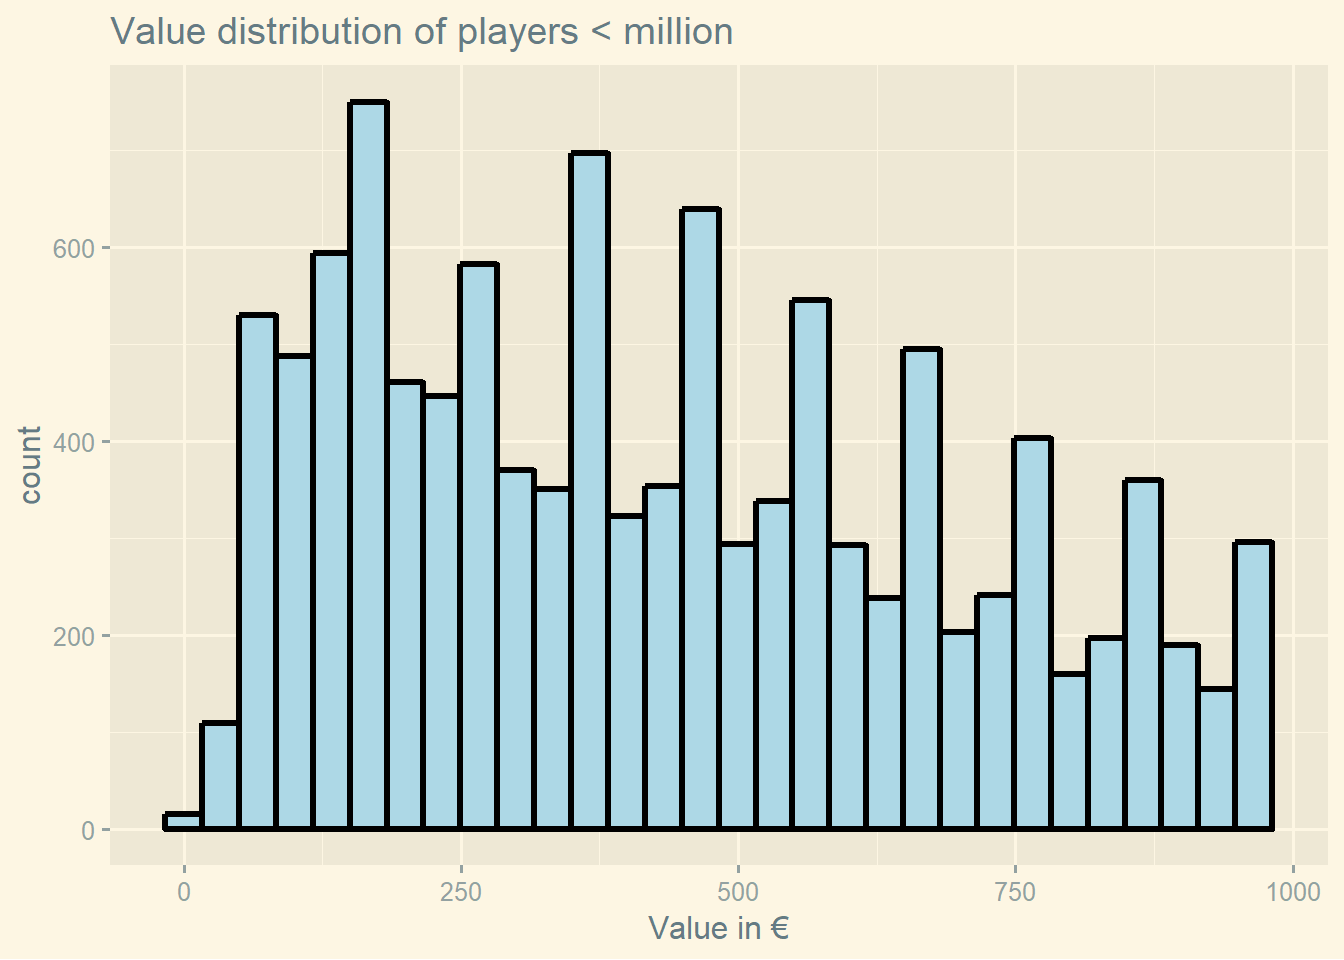
\includegraphics{football-cluster_files/figure-latex/unnamed-chunk-13-1.pdf}

\begin{Shaded}
\begin{Highlighting}[]
\NormalTok{fifa }\OperatorTok\StringTok{ }\KeywordTok{filter}\NormalTok{(value_k }\OperatorTok{>}\StringTok{ }\DecValTok{1000}\NormalTok{) }\OperatorTok
\StringTok{  }\KeywordTok{ggplot}\NormalTok{(}\KeywordTok{aes}\NormalTok{(}\DataTypeTok{x =}\NormalTok{ value_k)) }\OperatorTok{+}\StringTok{ }\KeywordTok{geom_histogram}\NormalTok{(}\DataTypeTok{size =} \FloatTok{1.2}\NormalTok{, }\DataTypeTok{fill =} \StringTok{"lightblue"}\NormalTok{, }\DataTypeTok{color =} \StringTok{'black'}\NormalTok{) }\OperatorTok{+}
\StringTok{  }\KeywordTok{labs}\NormalTok{(}\DataTypeTok{title =} \StringTok{"Value distribution of players >  1 million"}\NormalTok{, }\DataTypeTok{x =} \StringTok{"Value in €"}\NormalTok{)}
\end{Highlighting}
\end{Shaded}

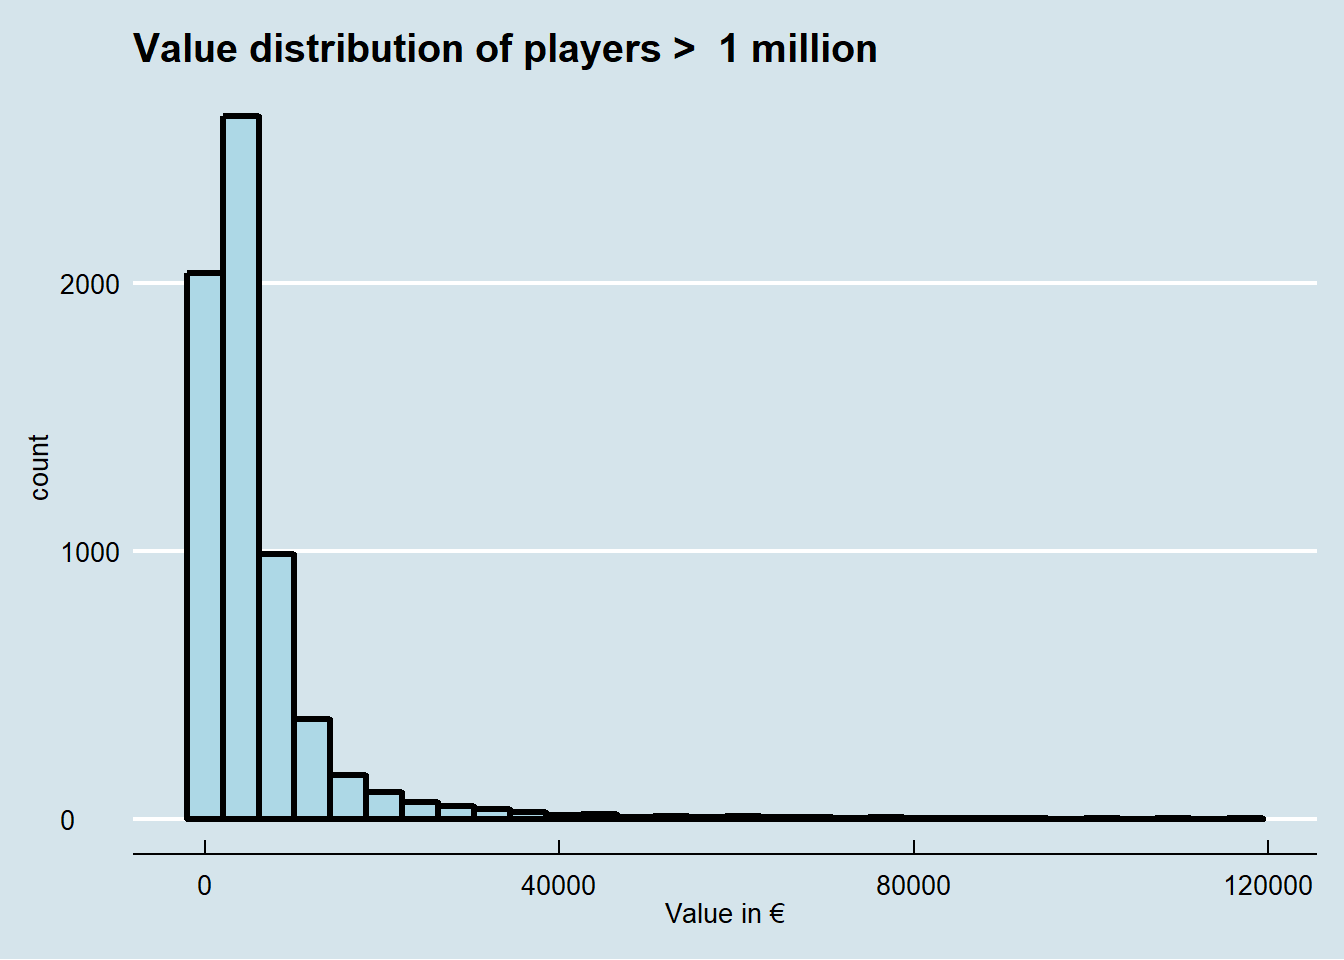
\includegraphics{football-cluster_files/figure-latex/unnamed-chunk-14-1.pdf}

\hypertarget{distribution-of-wage}{%
\subsection{Distribution of wage}\label{distribution-of-wage}}

\begin{Shaded}
\begin{Highlighting}[]
\NormalTok{fifa }\OperatorTok\StringTok{ }\KeywordTok{filter}\NormalTok{(Wage }\OperatorTok{<}\StringTok{ }\DecValTok{100}\NormalTok{) }\OperatorTok
\StringTok{  }\KeywordTok{ggplot}\NormalTok{(}\KeywordTok{aes}\NormalTok{(}\DataTypeTok{x =}\NormalTok{ Wage)) }\OperatorTok{+}\StringTok{ }\KeywordTok{geom_histogram}\NormalTok{(}\DataTypeTok{size =} \FloatTok{1.2}\NormalTok{, }\DataTypeTok{fill =} \StringTok{"lightblue"}\NormalTok{, }\DataTypeTok{color =} \StringTok{'black'}\NormalTok{) }\OperatorTok{+}\StringTok{ }\KeywordTok{labs}\NormalTok{(}\DataTypeTok{title =} \StringTok{"Distribution of wage < 100k €"}\NormalTok{)}
\end{Highlighting}
\end{Shaded}

\begin{verbatim}
## `stat_bin()` using `bins = 30`. Pick better value with `binwidth`.
\end{verbatim}

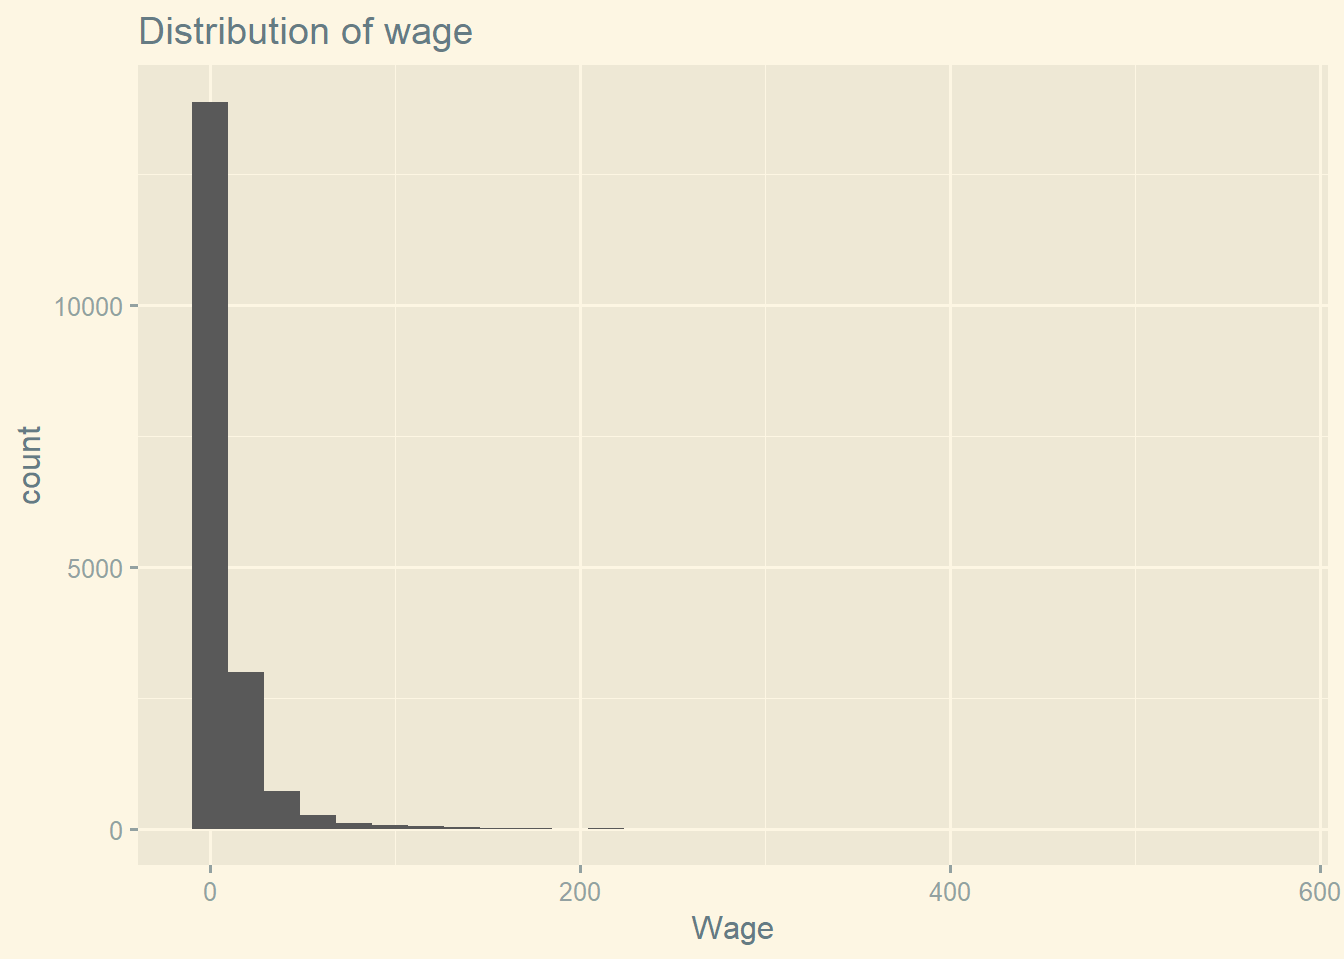
\includegraphics{football-cluster_files/figure-latex/unnamed-chunk-15-1.pdf}

\begin{Shaded}
\begin{Highlighting}[]
\NormalTok{fifa }\OperatorTok\StringTok{ }\KeywordTok{filter}\NormalTok{(Wage }\OperatorTok{>}\StringTok{ }\DecValTok{100}\NormalTok{) }\OperatorTok
\StringTok{  }\KeywordTok{ggplot}\NormalTok{(}\KeywordTok{aes}\NormalTok{(}\DataTypeTok{x =}\NormalTok{ Wage)) }\OperatorTok{+}\StringTok{ }\KeywordTok{geom_histogram}\NormalTok{(}\DataTypeTok{size =} \FloatTok{1.2}\NormalTok{, }\DataTypeTok{fill =} \StringTok{"lightblue"}\NormalTok{, }\DataTypeTok{color =} \StringTok{'black'}\NormalTok{) }\OperatorTok{+}\StringTok{ }\KeywordTok{labs}\NormalTok{(}\DataTypeTok{title =} \StringTok{"Distribution of wage > 100k €"}\NormalTok{)}
\end{Highlighting}
\end{Shaded}

\begin{verbatim}
## `stat_bin()` using `bins = 30`. Pick better value with `binwidth`.
\end{verbatim}

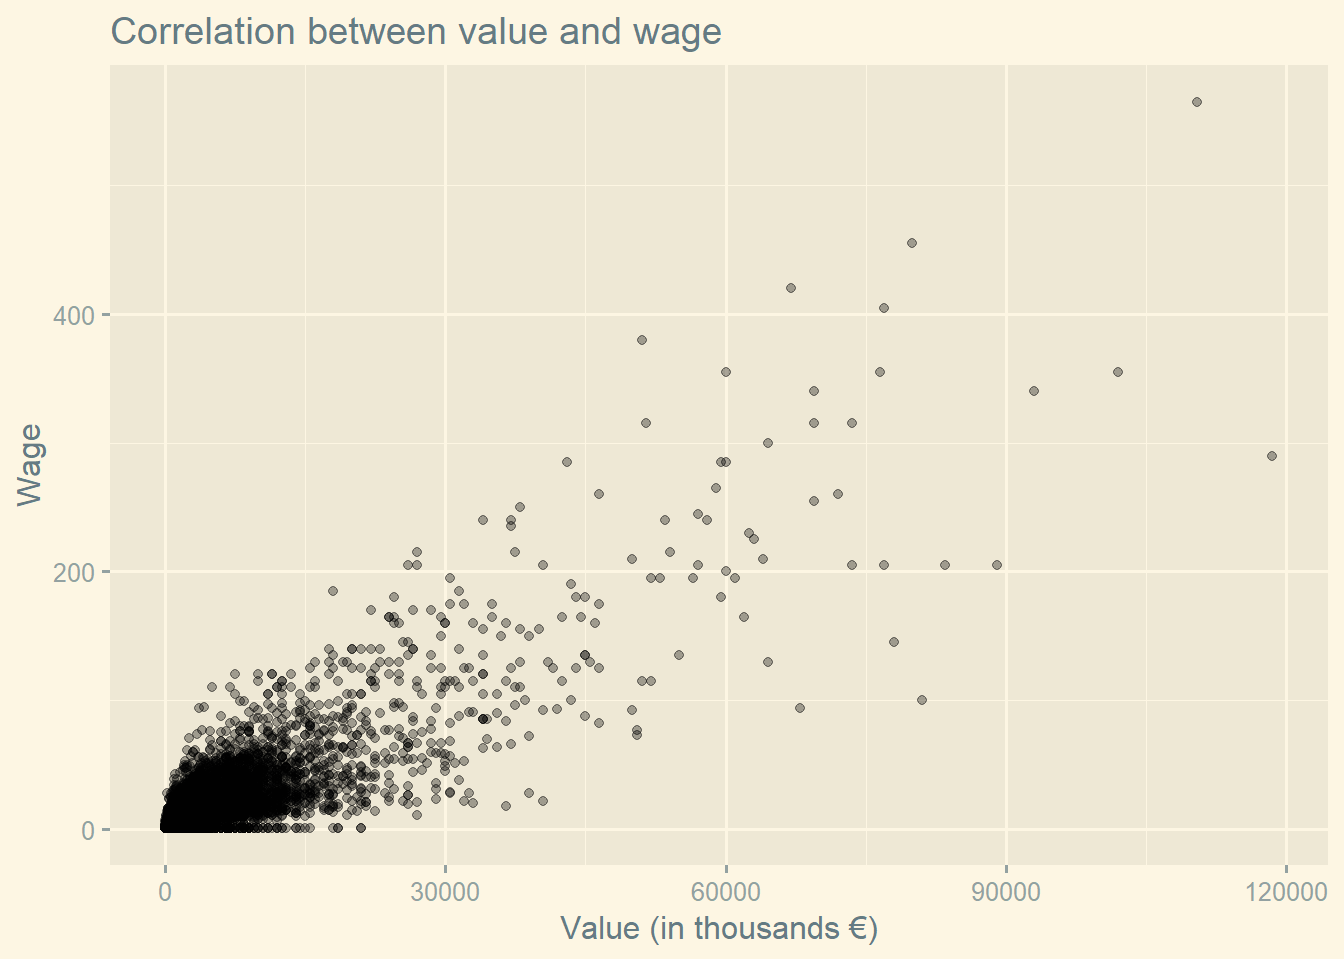
\includegraphics{football-cluster_files/figure-latex/unnamed-chunk-16-1.pdf}
\#\#\# Correlation between wage and value

\begin{Shaded}
\begin{Highlighting}[]
\NormalTok{fifa }\OperatorTok
\StringTok{  }\KeywordTok{ggplot}\NormalTok{(}\KeywordTok{aes}\NormalTok{(}\DataTypeTok{x =}\NormalTok{ value_k, }\DataTypeTok{y =}\NormalTok{ Wage)) }\OperatorTok{+}
\StringTok{  }\KeywordTok{geom_point}\NormalTok{(}\DataTypeTok{alpha =} \DecValTok{1}\OperatorTok{/}\DecValTok{3}\NormalTok{) }\OperatorTok{+}\StringTok{ }\KeywordTok{labs}\NormalTok{(}\DataTypeTok{title =} \StringTok{"Correlation between value and wage"}\NormalTok{, }\DataTypeTok{x =} \StringTok{"Value (in thousands €)"}\NormalTok{)}
\end{Highlighting}
\end{Shaded}

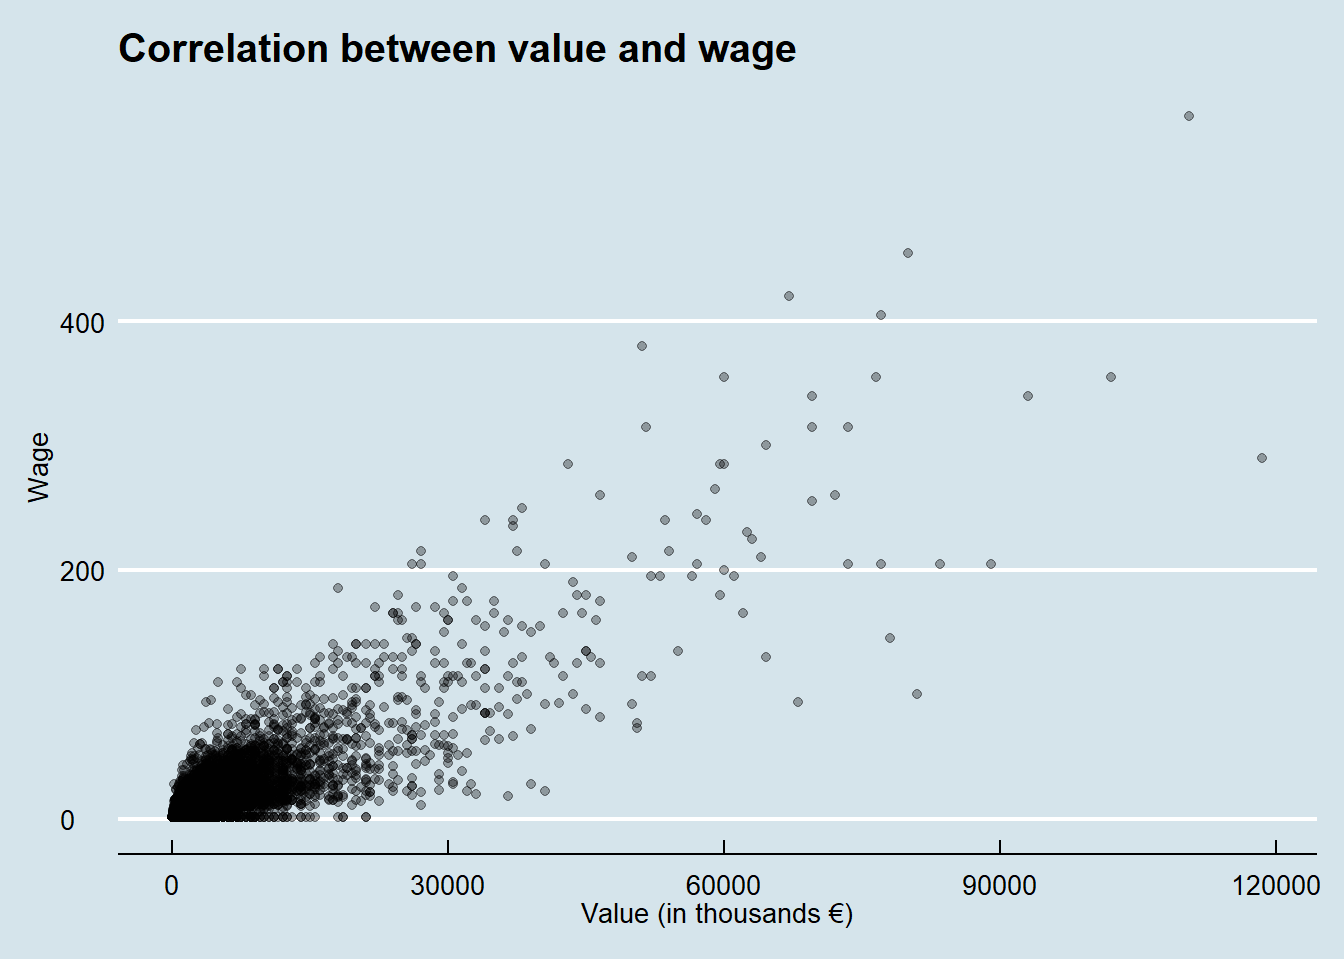
\includegraphics{football-cluster_files/figure-latex/unnamed-chunk-17-1.pdf}

\hypertarget{time-spent-in-current-club}{%
\subsection{Time spent in current
club}\label{time-spent-in-current-club}}

\begin{Shaded}
\begin{Highlighting}[]
\NormalTok{fifa <-}\StringTok{ }\NormalTok{fifa }\OperatorTok\StringTok{ }
\StringTok{  }\KeywordTok{mutate}\NormalTok{(}\DataTypeTok{months_in_current_club =} \KeywordTok{interval}\NormalTok{(Joined, }\KeywordTok{ymd}\NormalTok{(}\DecValTok{2019}\NormalTok{, }\DataTypeTok{truncated =}\NormalTok{ 2L))}\OperatorTok{/}\KeywordTok{months}\NormalTok{(}\DecValTok{1}\NormalTok{))}
\end{Highlighting}
\end{Shaded}

\hypertarget{link-between-time-spent-in-current-club-and-wage}{%
\subsubsection{Link between time spent in current club and
wage}\label{link-between-time-spent-in-current-club-and-wage}}

\begin{Shaded}
\begin{Highlighting}[]
\NormalTok{fifa }\OperatorTok
\StringTok{  }\KeywordTok{ggplot}\NormalTok{(}\KeywordTok{aes}\NormalTok{(}\DataTypeTok{x =}\NormalTok{ months_in_current_club, }\DataTypeTok{y =}\NormalTok{ Wage)) }\OperatorTok{+}
\StringTok{  }\KeywordTok{geom_point}\NormalTok{() }\OperatorTok{+}\StringTok{ }\KeywordTok{labs}\NormalTok{(}\DataTypeTok{x =} \StringTok{"Number of months"}\NormalTok{, }\DataTypeTok{y =} \StringTok{"Wage (thousands €)"}\NormalTok{)}
\end{Highlighting}
\end{Shaded}

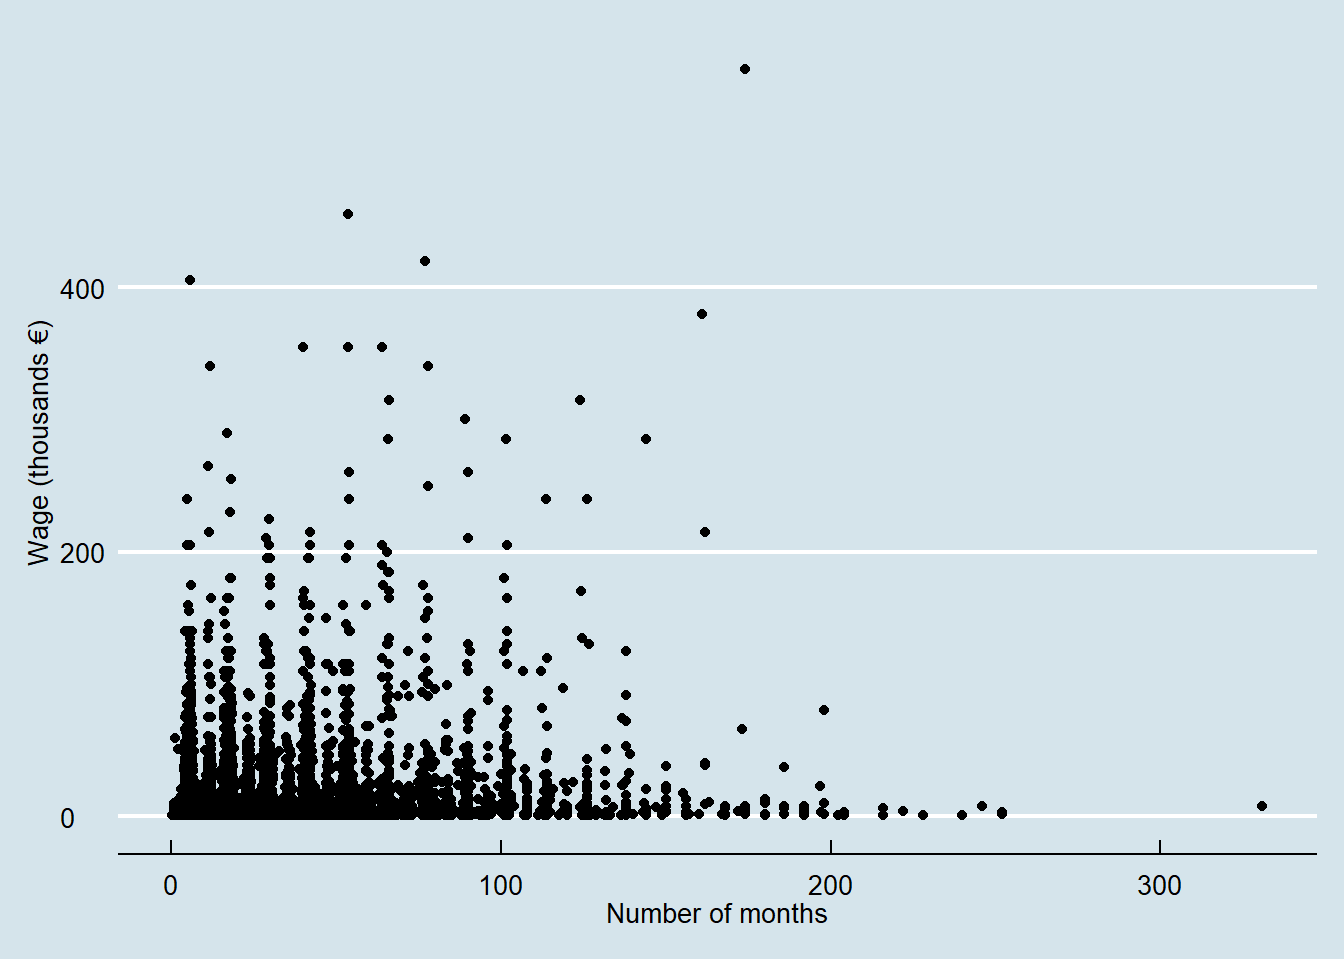
\includegraphics{football-cluster_files/figure-latex/unnamed-chunk-19-1.pdf}

There is not obvious relationship between time spent in a club and the
wage.

\hypertarget{what-are-the-top-nationality-of-the-players}{%
\subsection{What are the top nationality of the
players}\label{what-are-the-top-nationality-of-the-players}}

\begin{Shaded}
\begin{Highlighting}[]
\NormalTok{fifa }\OperatorTok\StringTok{ }\KeywordTok{group_by}\NormalTok{(Nationality) }\OperatorTok
\StringTok{  }\KeywordTok{summarize}\NormalTok{(}\DataTypeTok{count =} \KeywordTok{n}\NormalTok{()) }\OperatorTok
\StringTok{  }\KeywordTok{treemap}\NormalTok{(}\DataTypeTok{index =} \StringTok{"Nationality"}\NormalTok{, }\DataTypeTok{vSize =} \StringTok{"count"}\NormalTok{, }\DataTypeTok{title =} \StringTok{"Nationality of players"}\NormalTok{)}
\end{Highlighting}
\end{Shaded}

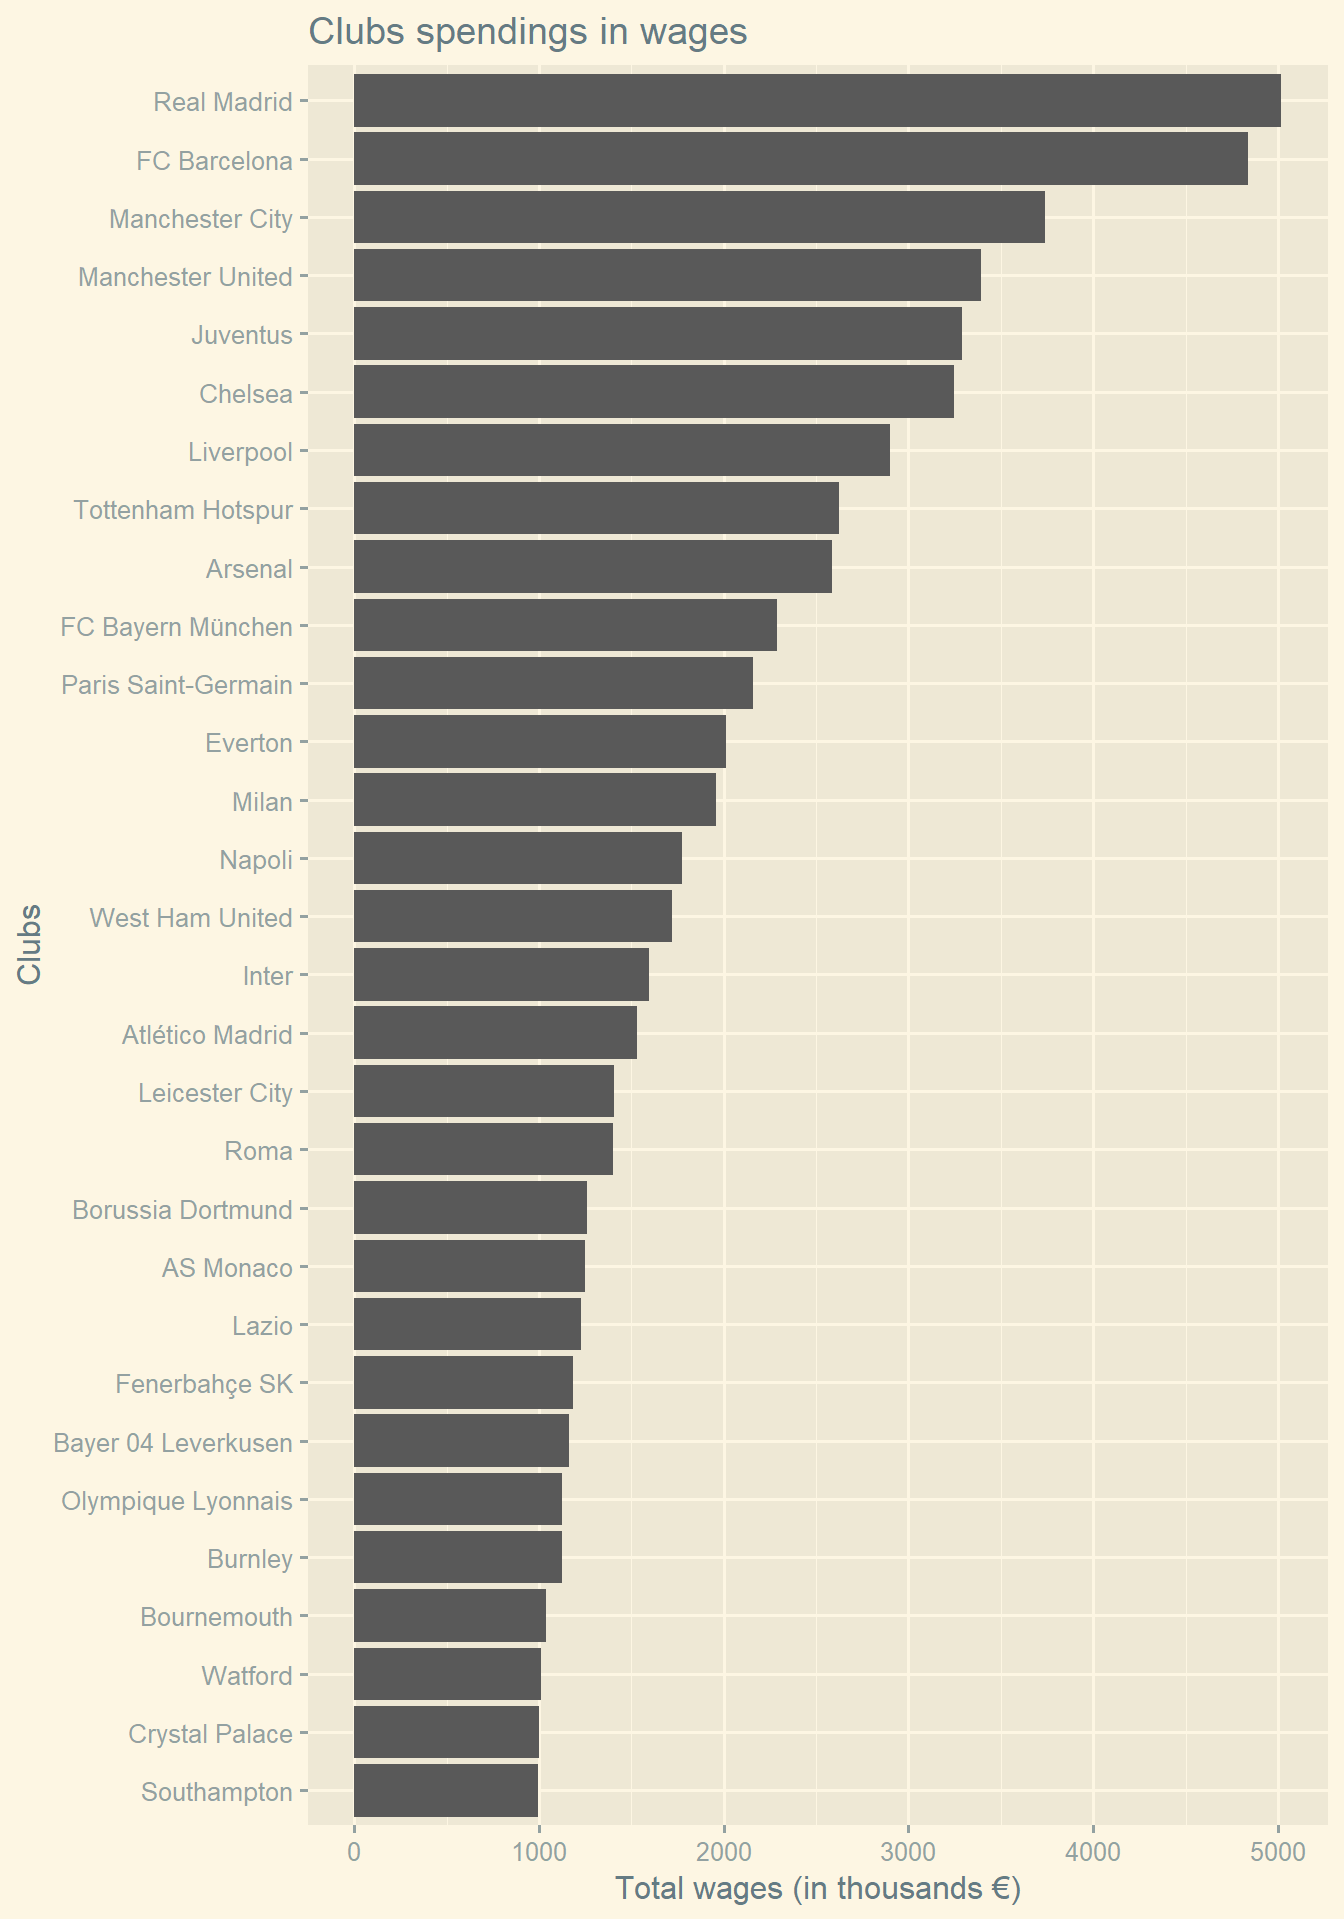
\includegraphics{football-cluster_files/figure-latex/unnamed-chunk-20-1.pdf}

This quite interesting. Out of the Fist five nationalities, 4 are
European countries. Football is really popular in Europe in Europe.

\hypertarget{which-clubs-have-the-highest-spendings-for-their-players}{%
\subsection{Which clubs have the highest spendings for their
players}\label{which-clubs-have-the-highest-spendings-for-their-players}}

\begin{Shaded}
\begin{Highlighting}[]
\NormalTok{fifa }\OperatorTok
\StringTok{  }\KeywordTok{group_by}\NormalTok{(Club) }\OperatorTok\StringTok{ }\KeywordTok{summarize}\NormalTok{(}\DataTypeTok{spending =} \KeywordTok{sum}\NormalTok{(Wage)) }\OperatorTok\StringTok{ }\KeywordTok{top_n}\NormalTok{(}\DecValTok{35}\NormalTok{) }\OperatorTok
\StringTok{  }\KeywordTok{ggplot}\NormalTok{(}\KeywordTok{aes}\NormalTok{(}\DataTypeTok{y =}\NormalTok{ spending, }\DataTypeTok{x =} \KeywordTok{reorder}\NormalTok{(Club, spending))) }\OperatorTok{+}\StringTok{ }
\StringTok{           }\KeywordTok{geom_bar}\NormalTok{(}\DataTypeTok{stat =} \StringTok{"identity"}\NormalTok{) }\OperatorTok{+}\StringTok{ }\KeywordTok{coord_flip}\NormalTok{() }\OperatorTok{+}\StringTok{ }
\StringTok{  }\KeywordTok{labs}\NormalTok{(}\DataTypeTok{y =} \StringTok{"Total wages (in thousands €)"}\NormalTok{, }\DataTypeTok{x =} \StringTok{"Clubs"}\NormalTok{, }\DataTypeTok{title =} \StringTok{"Clubs spendings in wages"}\NormalTok{)}
\end{Highlighting}
\end{Shaded}

\begin{verbatim}
## Selecting by spending
\end{verbatim}

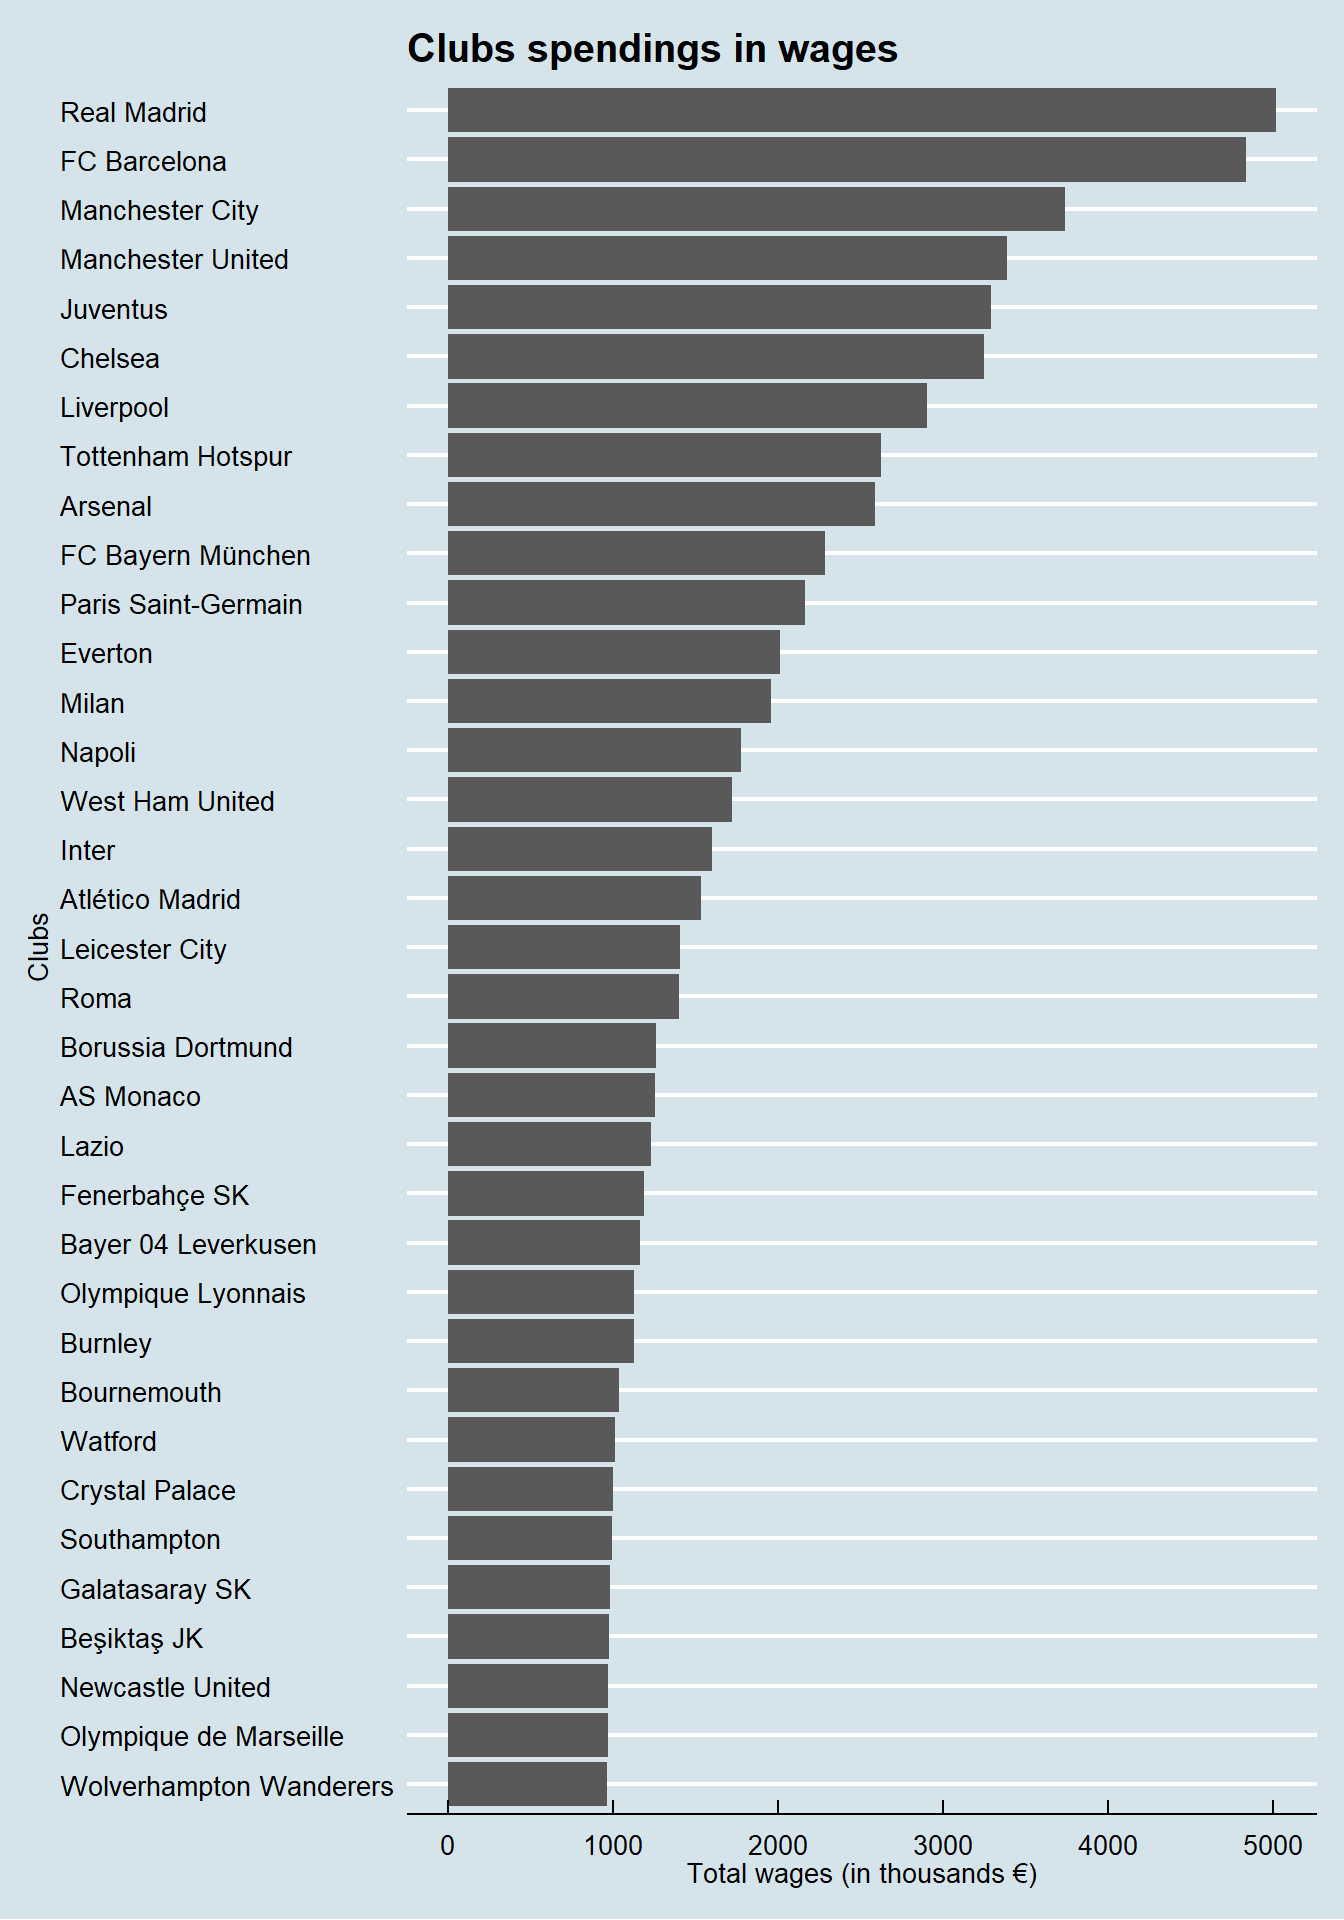
\includegraphics{football-cluster_files/figure-latex/unnamed-chunk-21-1.pdf}

\hypertarget{cluster-analysis}{%
\section{Cluster Analysis}\label{cluster-analysis}}

In this section we want to study how can we gather the players based on
their characteristics. We will use all the technical columns.

\begin{Shaded}
\begin{Highlighting}[]
\KeywordTok{library}\NormalTok{(FactoMineR)}
\KeywordTok{library}\NormalTok{(factoextra)}
\end{Highlighting}
\end{Shaded}

Since I am not a football professional I'm going to use the columns that
mean something in this cluster analysis. Let's select the columns

\begin{Shaded}
\begin{Highlighting}[]
\KeywordTok{head}\NormalTok{(fifa)}
\end{Highlighting}
\end{Shaded}

\begin{verbatim}
## # A tibble: 6 x 92
##      X1     ID Name    Age Photo Nationality Flag  Overall Potential Club 
##   <dbl>  <dbl> <chr> <dbl> <chr> <chr>       <chr>   <dbl>     <dbl> <chr>
## 1     0 158023 L. M~    31 http~ Argentina   http~      94        94 FC B~
## 2     1  20801 Cris~    33 http~ Portugal    http~      94        94 Juve~
## 3     2 190871 Neym~    26 http~ Brazil      http~      92        93 Pari~
## 4     3 193080 De G~    27 http~ Spain       http~      91        93 Manc~
## 5     4 192985 K. D~    27 http~ Belgium     http~      91        92 Manc~
## 6     5 183277 E. H~    27 http~ Belgium     http~      91        91 Chel~
## # ... with 82 more variables: `Club Logo` <chr>, raw_value <chr>,
## #   unit_value <chr>, Wage <dbl>, Special <dbl>, `Preferred Foot` <chr>,
## #   `International Reputation` <dbl>, `Weak Foot` <dbl>, `Skill
## #   Moves` <dbl>, `Work Rate` <chr>, `Body Type` <chr>, `Real Face` <chr>,
## #   Position <chr>, `Jersey Number` <dbl>, Joined <date>, `Loaned
## #   From` <chr>, Contract_Validity <date>, Height <chr>, Weight <chr>,
## #   LS <chr>, ST <chr>, RS <chr>, LW <chr>, LF <chr>, CF <chr>, RF <chr>,
## #   RW <chr>, LAM <chr>, CAM <chr>, RAM <chr>, LM <chr>, LCM <chr>,
## #   CM <chr>, RCM <chr>, RM <chr>, LWB <chr>, LDM <chr>, CDM <chr>,
## #   RDM <chr>, RWB <chr>, LB <chr>, LCB <chr>, CB <chr>, RCB <chr>,
## #   RB <chr>, Crossing <dbl>, Finishing <dbl>, HeadingAccuracy <dbl>,
## #   ShortPassing <dbl>, Volleys <dbl>, Dribbling <dbl>, Curve <dbl>,
## #   FKAccuracy <dbl>, LongPassing <dbl>, BallControl <dbl>,
## #   Acceleration <dbl>, SprintSpeed <dbl>, Agility <dbl>, Reactions <dbl>,
## #   Balance <dbl>, ShotPower <dbl>, Jumping <dbl>, Stamina <dbl>,
## #   Strength <dbl>, LongShots <dbl>, Aggression <dbl>,
## #   Interceptions <dbl>, Positioning <dbl>, Vision <dbl>, Penalties <dbl>,
## #   Composure <dbl>, Marking <dbl>, StandingTackle <dbl>,
## #   SlidingTackle <dbl>, GKDiving <dbl>, GKHandling <dbl>,
## #   GKKicking <dbl>, GKPositioning <dbl>, GKReflexes <dbl>, `Release
## #   Clause` <chr>, value_k <dbl>, months_in_current_club <dbl>
\end{verbatim}

\begin{Shaded}
\begin{Highlighting}[]
\NormalTok{pca_data <-}\StringTok{ }\NormalTok{fifa[}\KeywordTok{c}\NormalTok{(}\DecValTok{3}\OperatorTok{:}\DecValTok{4}\NormalTok{,}\DecValTok{56}\OperatorTok{:}\DecValTok{89}\NormalTok{)]}
\end{Highlighting}
\end{Shaded}

\begin{Shaded}
\begin{Highlighting}[]
\CommentTok{# Remove duplicate players}
\NormalTok{pca_data <-}\StringTok{ }\NormalTok{pca_data }\OperatorTok\StringTok{ }\KeywordTok{filter}\NormalTok{(}\OperatorTok{!}\KeywordTok{duplicated}\NormalTok{(Name))}
\end{Highlighting}
\end{Shaded}

Clean the missing values

\begin{Shaded}
\begin{Highlighting}[]
\NormalTok{pca_data <-}\StringTok{ }\KeywordTok{na.omit}\NormalTok{(pca_data)}
\NormalTok{pca_data <-}\StringTok{ }\KeywordTok{data.frame}\NormalTok{(pca_data, }\DataTypeTok{row.names =} \DecValTok{1}\NormalTok{)}
\end{Highlighting}
\end{Shaded}

\begin{Shaded}
\begin{Highlighting}[]
\KeywordTok{head}\NormalTok{(pca_data)}
\end{Highlighting}
\end{Shaded}

\begin{verbatim}
##                   Age Crossing Finishing HeadingAccuracy ShortPassing
## L. Messi           31       84        95              70           90
## Cristiano Ronaldo  33       84        94              89           81
## Neymar Jr          26       79        87              62           84
## De Gea             27       17        13              21           50
## K. De Bruyne       27       93        82              55           92
## E. Hazard          27       81        84              61           89
##                   Volleys Dribbling Curve FKAccuracy LongPassing
## L. Messi               86        97    93         94          87
## Cristiano Ronaldo      87        88    81         76          77
## Neymar Jr              84        96    88         87          78
## De Gea                 13        18    21         19          51
## K. De Bruyne           82        86    85         83          91
## E. Hazard              80        95    83         79          83
##                   BallControl Acceleration SprintSpeed Agility Reactions
## L. Messi                   96           91          86      91        95
## Cristiano Ronaldo          94           89          91      87        96
## Neymar Jr                  95           94          90      96        94
## De Gea                     42           57          58      60        90
## K. De Bruyne               91           78          76      79        91
## E. Hazard                  94           94          88      95        90
##                   Balance ShotPower Jumping Stamina Strength LongShots
## L. Messi               95        85      68      72       59        94
## Cristiano Ronaldo      70        95      95      88       79        93
## Neymar Jr              84        80      61      81       49        82
## De Gea                 43        31      67      43       64        12
## K. De Bruyne           77        91      63      90       75        91
## E. Hazard              94        82      56      83       66        80
##                   Aggression Interceptions Positioning Vision Penalties
## L. Messi                  48            22          94     94        75
## Cristiano Ronaldo         63            29          95     82        85
## Neymar Jr                 56            36          89     87        81
## De Gea                    38            30          12     68        40
## K. De Bruyne              76            61          87     94        79
## E. Hazard                 54            41          87     89        86
##                   Composure Marking StandingTackle SlidingTackle GKDiving
## L. Messi                 96      33             28            26        6
## Cristiano Ronaldo        95      28             31            23        7
## Neymar Jr                94      27             24            33        9
## De Gea                   68      15             21            13       90
## K. De Bruyne             88      68             58            51       15
## E. Hazard                91      34             27            22       11
##                   GKHandling GKKicking GKPositioning GKReflexes
## L. Messi                  11        15            14          8
## Cristiano Ronaldo         11        15            14         11
## Neymar Jr                  9        15            15         11
## De Gea                    85        87            88         94
## K. De Bruyne              13         5            10         13
## E. Hazard                 12         6             8          8
\end{verbatim}

\begin{Shaded}
\begin{Highlighting}[]
\NormalTok{pca <-}\StringTok{ }\KeywordTok{PCA}\NormalTok{(pca_data, }\DataTypeTok{quanti.sup =} \DecValTok{1}\NormalTok{)}
\end{Highlighting}
\end{Shaded}

\begin{verbatim}
## Warning in text.default(coo[labe != "", 1], y = coo[labe != "", 2], labels
## = labe[labe != : erreur de conversion de 'A. Coșelev' dans 'mbcsToSbcs' :
## le point est substitué pour <c8>
\end{verbatim}

\begin{verbatim}
## Warning in text.default(coo[labe != "", 1], y = coo[labe != "", 2], labels
## = labe[labe != : erreur de conversion de 'A. Coșelev' dans 'mbcsToSbcs' :
## le point est substitué pour <99>
\end{verbatim}

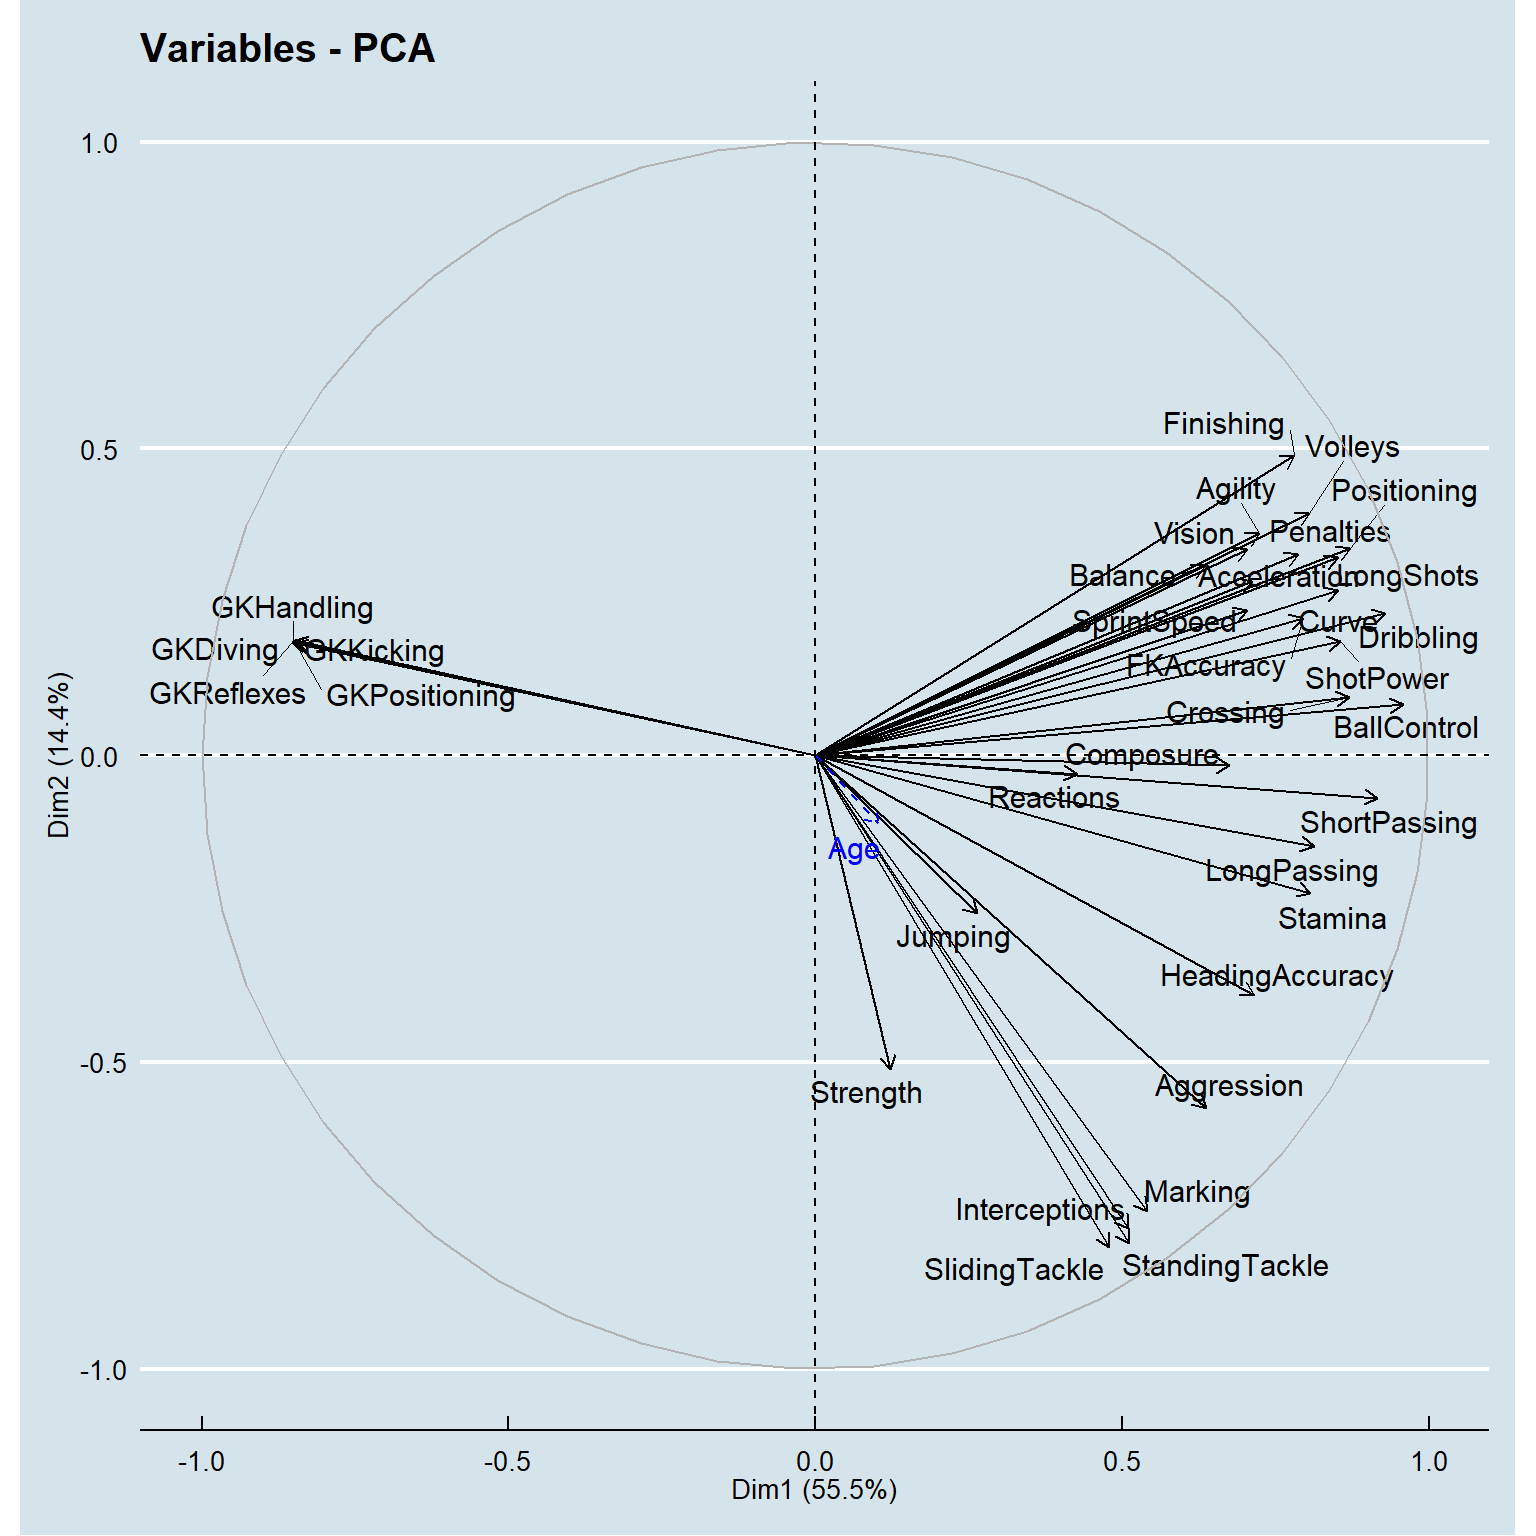
\includegraphics{football-cluster_files/figure-latex/unnamed-chunk-28-1.pdf}
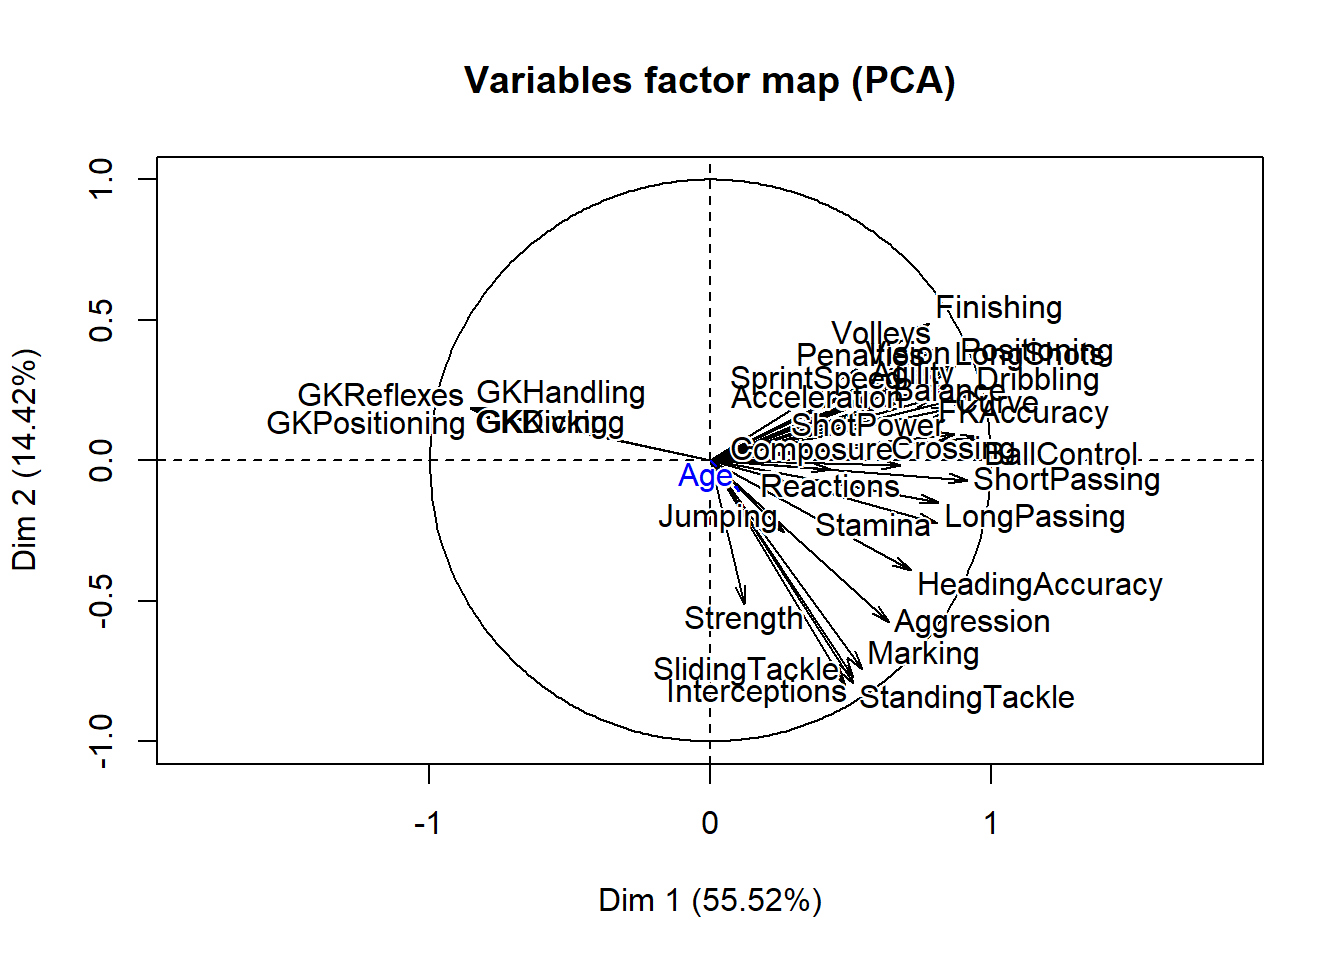
\includegraphics{football-cluster_files/figure-latex/unnamed-chunk-28-2.pdf}

Let's now try to see how correlated are the variables and discover how
they separate the players.

\begin{Shaded}
\begin{Highlighting}[]
\KeywordTok{fviz_pca_var}\NormalTok{(pca, }\DataTypeTok{repel =}\NormalTok{ T) }\OperatorTok{+}\StringTok{ }\KeywordTok{theme_economist}\NormalTok{()}
\end{Highlighting}
\end{Shaded}

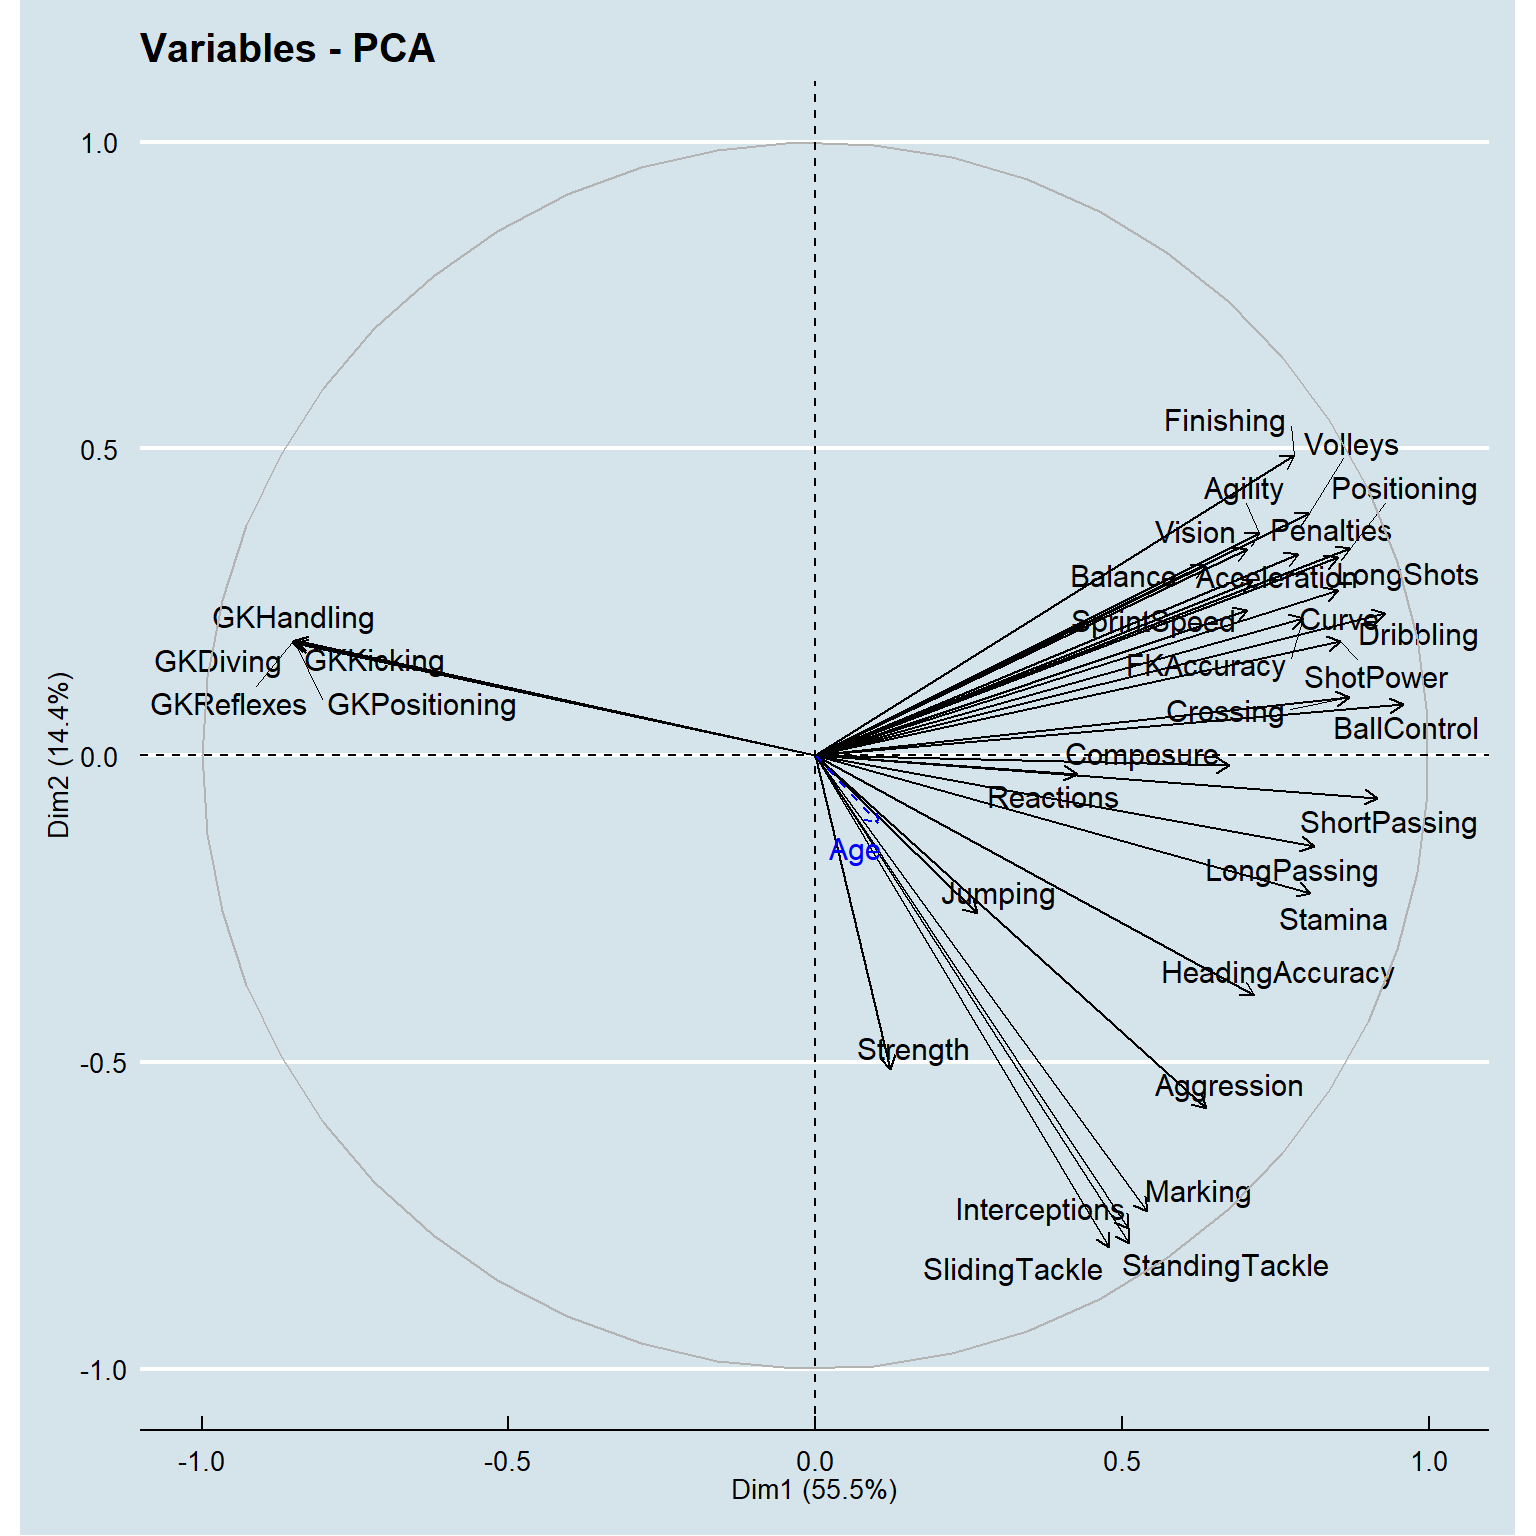
\includegraphics{football-cluster_files/figure-latex/unnamed-chunk-29-1.pdf}

\begin{Shaded}
\begin{Highlighting}[]
\KeywordTok{dimdesc}\NormalTok{(pca)}
\end{Highlighting}
\end{Shaded}

\begin{verbatim}
## $Dim.1
## $Dim.1$quanti
##                 correlation       p.value
## BallControl       0.9575674  0.000000e+00
## Dribbling         0.9292212  0.000000e+00
## ShortPassing      0.9163976  0.000000e+00
## Positioning       0.8718798  0.000000e+00
## Crossing          0.8705012  0.000000e+00
## ShotPower         0.8563707  0.000000e+00
## Curve             0.8522071  0.000000e+00
## LongShots         0.8517836  0.000000e+00
## LongPassing       0.8126963  0.000000e+00
## Stamina           0.8073784  0.000000e+00
## Volleys           0.8056571  0.000000e+00
## FKAccuracy        0.7951769  0.000000e+00
## Penalties         0.7871776  0.000000e+00
## Finishing         0.7807105  0.000000e+00
## Agility           0.7243417  0.000000e+00
## HeadingAccuracy   0.7159097  0.000000e+00
## Acceleration      0.7123085  0.000000e+00
## SprintSpeed       0.7041238  0.000000e+00
## Vision            0.7039064  0.000000e+00
## Composure         0.6750123  0.000000e+00
## Aggression        0.6369436  0.000000e+00
## Balance           0.6350150  0.000000e+00
## Marking           0.5407773  0.000000e+00
## StandingTackle    0.5111614  0.000000e+00
## Interceptions     0.5095279  0.000000e+00
## SlidingTackle     0.4793948  0.000000e+00
## Reactions         0.4262738  0.000000e+00
## Jumping           0.2632617 8.458303e-270
## Strength          0.1226311  1.883645e-58
## Age               0.1027927  1.652906e-41
## GKKicking        -0.8483274  0.000000e+00
## GKPositioning    -0.8484342  0.000000e+00
## GKHandling       -0.8517354  0.000000e+00
## GKReflexes       -0.8525332  0.000000e+00
## GKDiving         -0.8533499  0.000000e+00
## 
## 
## $Dim.2
## $Dim.2$quanti
##                 correlation       p.value
## Finishing        0.48869080  0.000000e+00
## Volleys          0.39497273  0.000000e+00
## Agility          0.36161221  0.000000e+00
## Positioning      0.33718933  0.000000e+00
## Vision           0.33672344  0.000000e+00
## Penalties        0.32794746  0.000000e+00
## LongShots        0.32309363  0.000000e+00
## Balance          0.30934699  0.000000e+00
## Acceleration     0.28467696 4.463986e-317
## Curve            0.26913331 2.457159e-282
## SprintSpeed      0.23622994 4.019428e-216
## Dribbling        0.23147968 2.312527e-207
## FKAccuracy       0.22333367 8.455848e-193
## GKKicking        0.18696811 1.054205e-134
## ShotPower        0.18605096 2.212049e-133
## GKHandling       0.18586050 4.153619e-133
## GKDiving         0.18469723 1.919634e-131
## GKReflexes       0.18462331 2.446956e-131
## GKPositioning    0.18245441 2.894091e-128
## Crossing         0.09501422  1.090711e-35
## BallControl      0.08345967  6.815662e-28
## Composure       -0.01643873  3.134159e-02
## Reactions       -0.03010491  8.047868e-05
## ShortPassing    -0.06956196  7.525288e-20
## Age             -0.11049258  1.004341e-47
## LongPassing     -0.14743043  6.184010e-84
## Stamina         -0.22397254 6.395073e-194
## Jumping         -0.25648884 9.891799e-256
## HeadingAccuracy -0.39038523  0.000000e+00
## Strength        -0.51113647  0.000000e+00
## Aggression      -0.57430161  0.000000e+00
## Marking         -0.74305466  0.000000e+00
## Interceptions   -0.77149466  0.000000e+00
## StandingTackle  -0.79446128  0.000000e+00
## SlidingTackle   -0.80109110  0.000000e+00
## 
## 
## $Dim.3
## $Dim.3$quanti
##                correlation       p.value
## Reactions       0.73323051  0.000000e+00
## Age             0.55111367  0.000000e+00
## Composure       0.53883124  0.000000e+00
## GKPositioning   0.41000841  0.000000e+00
## GKHandling      0.40447867  0.000000e+00
## GKReflexes      0.40429174  0.000000e+00
## GKKicking       0.40274211  0.000000e+00
## GKDiving        0.40114161  0.000000e+00
## Strength        0.38320668  0.000000e+00
## Vision          0.37647732  0.000000e+00
## LongPassing     0.24431357 1.735274e-231
## FKAccuracy      0.20506235 3.258515e-162
## LongShots       0.17944771 4.544011e-124
## ShotPower       0.17399244 1.206321e-116
## Aggression      0.17287201 3.768740e-115
## Curve           0.15234669  1.456918e-89
## ShortPassing    0.14868943  2.335257e-85
## Volleys         0.14289355  6.527233e-79
## Interceptions   0.11498692  1.455053e-51
## Jumping         0.09745726  1.818163e-37
## Penalties       0.08770203  1.226461e-30
## Finishing       0.06213573  3.817631e-16
## BallControl     0.04354398  1.166468e-08
## Crossing        0.04175925  4.486744e-08
## Positioning     0.03431513  6.966596e-06
## Marking         0.02828461  2.118418e-04
## StandingTackle  0.02147269  4.922562e-03
## Stamina        -0.02418791  1.536283e-03
## Dribbling      -0.03738368  9.735851e-07
## Agility        -0.14372548  8.049441e-80
## Balance        -0.26358489 1.759919e-270
## SprintSpeed    -0.29679997  0.000000e+00
## Acceleration   -0.30572583  0.000000e+00
\end{verbatim}

\begin{Shaded}
\begin{Highlighting}[]
\KeywordTok{fviz_pca_contrib}\NormalTok{(pca, }\DataTypeTok{choice =} \StringTok{"var"}\NormalTok{)}
\end{Highlighting}
\end{Shaded}

\begin{verbatim}
## Warning in fviz_pca_contrib(pca, choice = "var"): The function
## fviz_pca_contrib() is deprecated. Please use the function fviz_contrib()
## which can handle outputs of PCA, CA and MCA functions.
\end{verbatim}

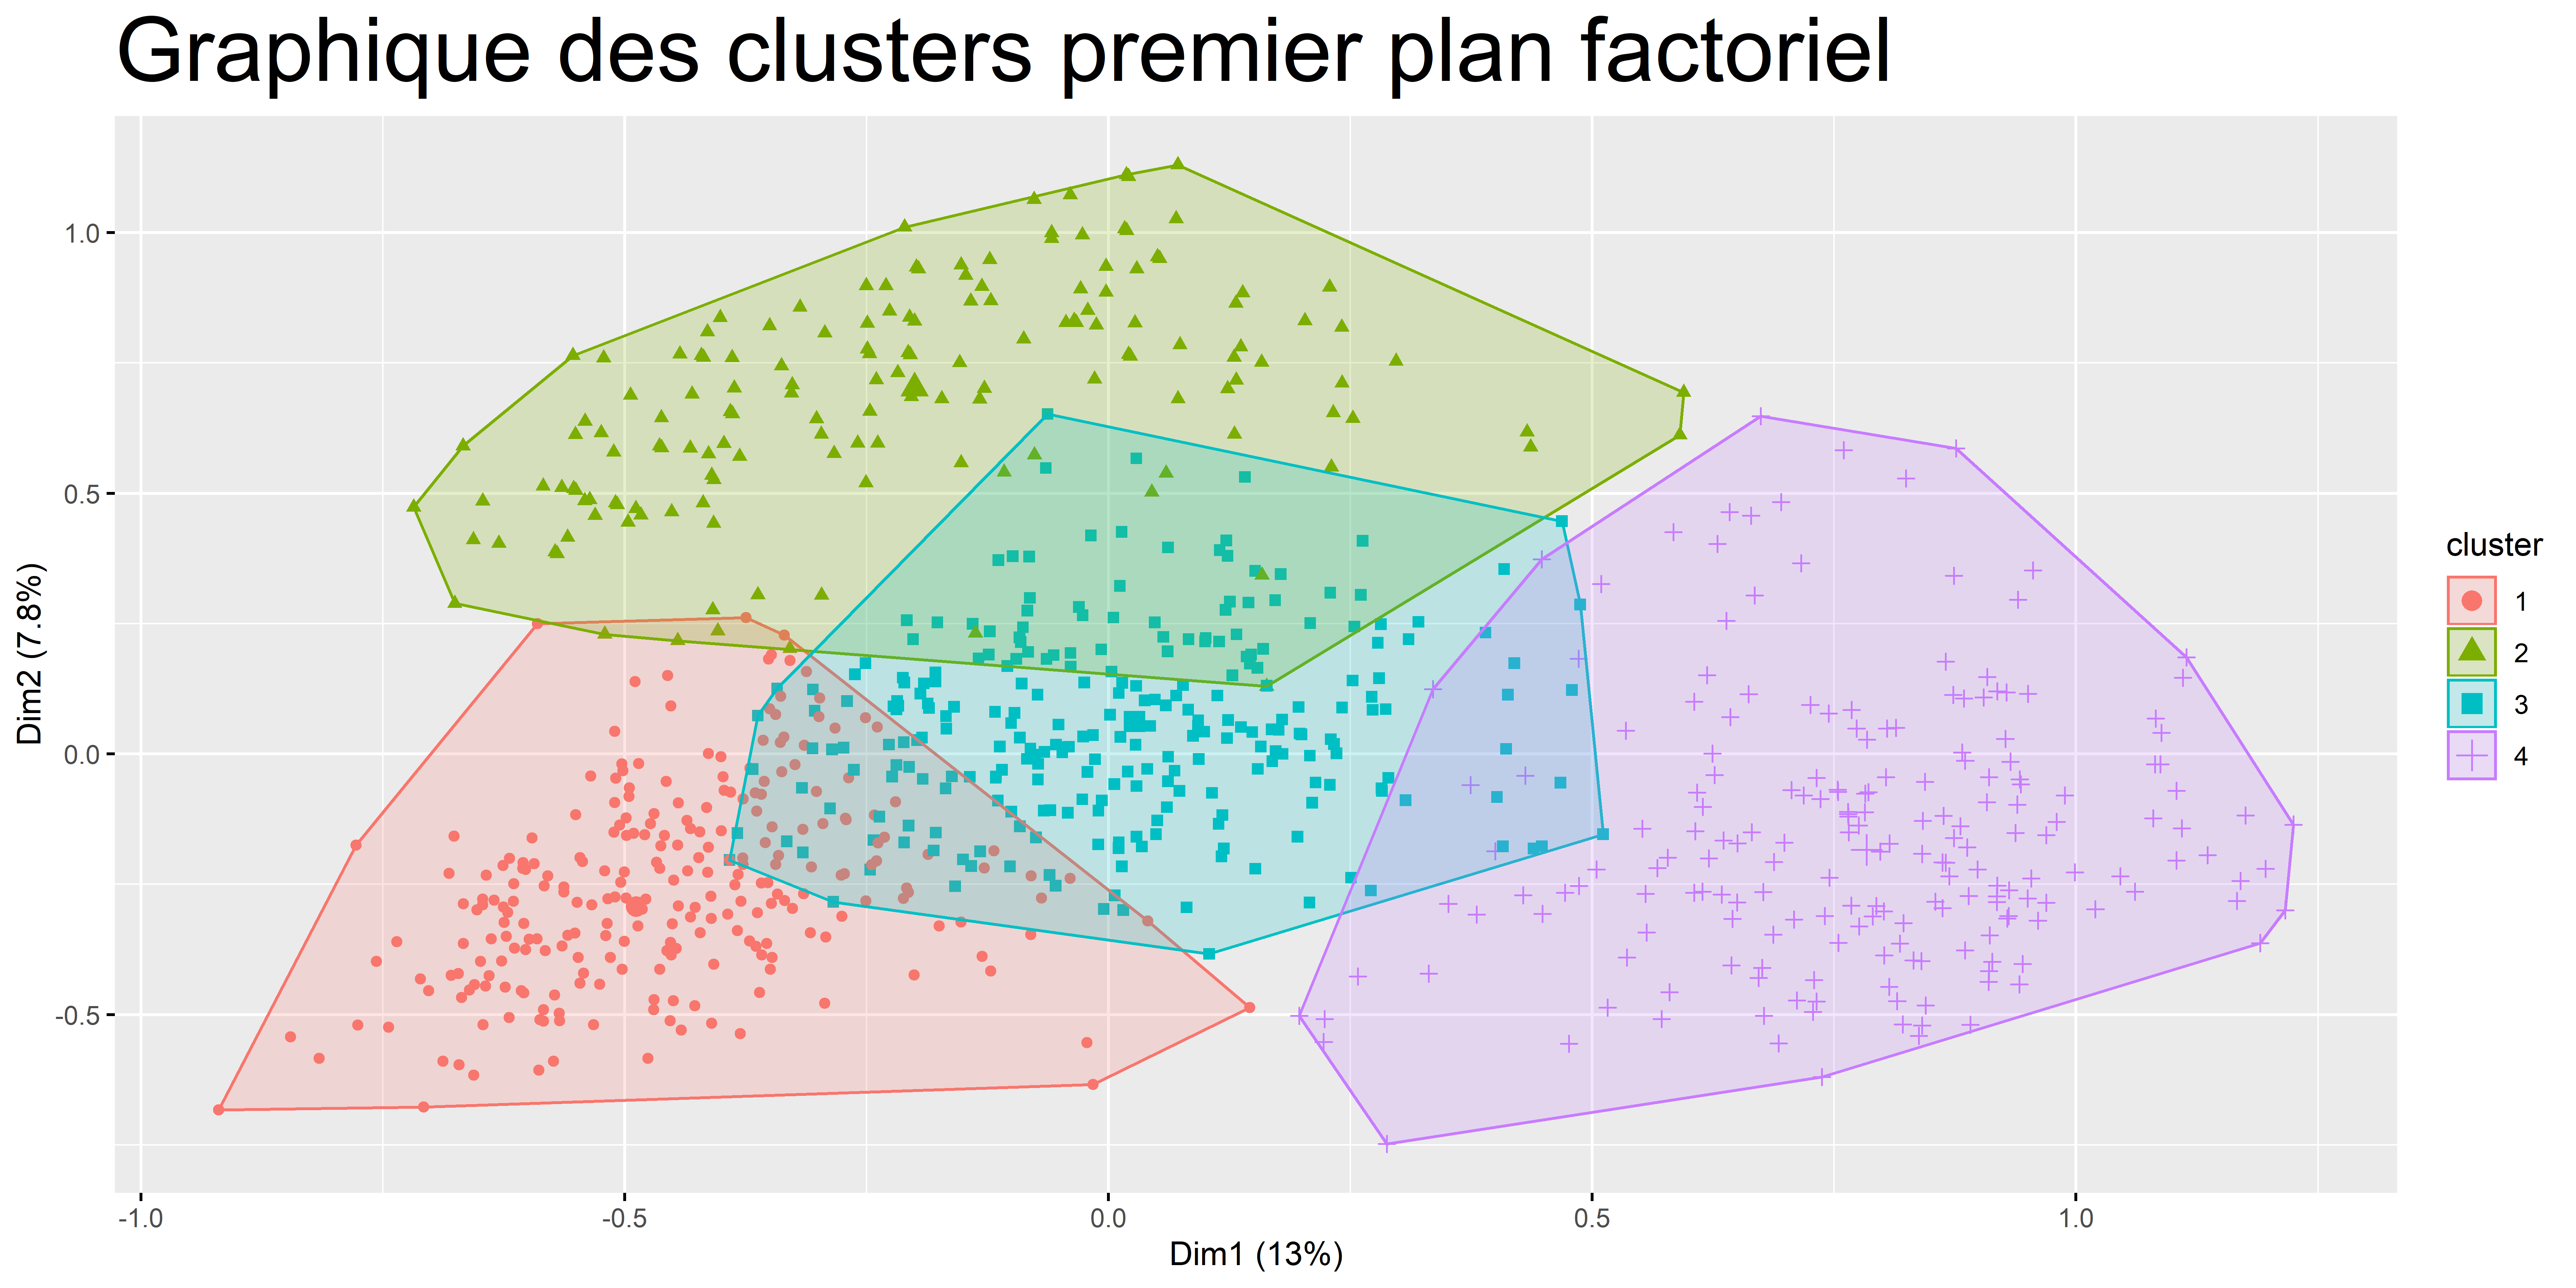
\includegraphics{football-cluster_files/figure-latex/unnamed-chunk-31-1.pdf}

\begin{Shaded}
\begin{Highlighting}[]
\KeywordTok{fviz_pca_contrib}\NormalTok{(pca, }\DataTypeTok{choice =} \StringTok{"var"}\NormalTok{, }\DataTypeTok{axes =} \DecValTok{2}\NormalTok{)}
\end{Highlighting}
\end{Shaded}

\begin{verbatim}
## Warning in fviz_pca_contrib(pca, choice = "var", axes = 2): The function
## fviz_pca_contrib() is deprecated. Please use the function fviz_contrib()
## which can handle outputs of PCA, CA and MCA functions.
\end{verbatim}

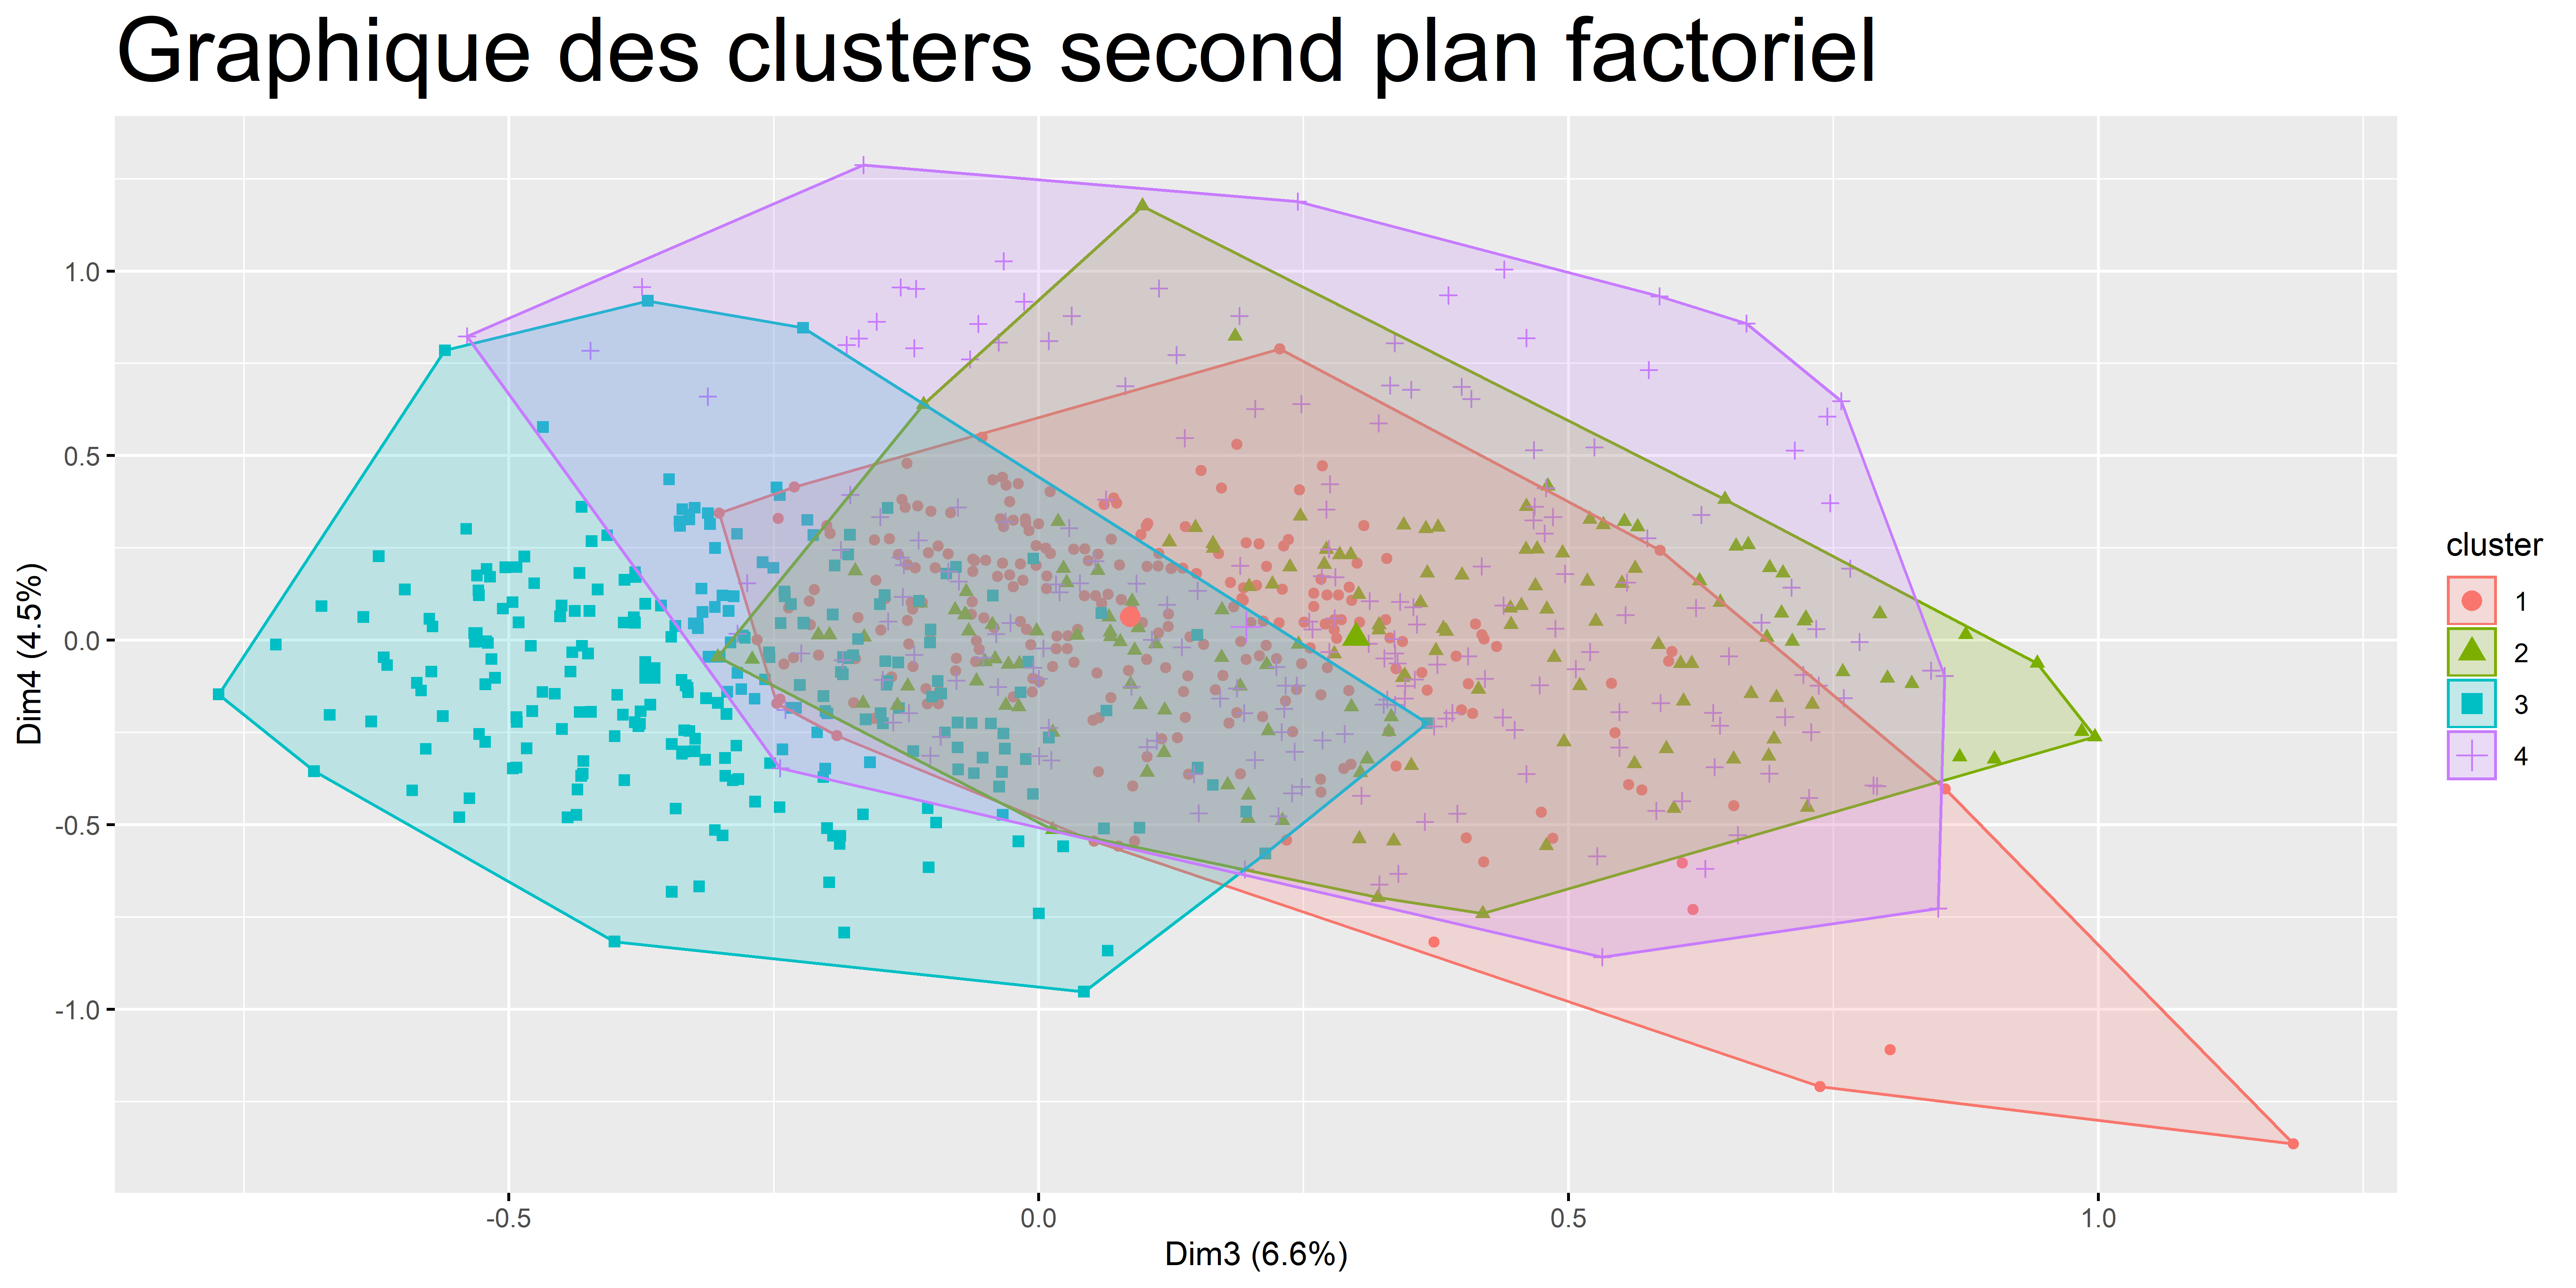
\includegraphics{football-cluster_files/figure-latex/unnamed-chunk-32-1.pdf}

\begin{Shaded}
\begin{Highlighting}[]
\KeywordTok{fviz_pca_ind}\NormalTok{(pca, }\DataTypeTok{geom =} \StringTok{"point"}\NormalTok{, }\DataTypeTok{alpha.ind =} \StringTok{"contrib"}\NormalTok{, }\DataTypeTok{addEllipses =}\NormalTok{ T) }\OperatorTok{+}\StringTok{ }\KeywordTok{theme_economist}\NormalTok{()}
\end{Highlighting}
\end{Shaded}

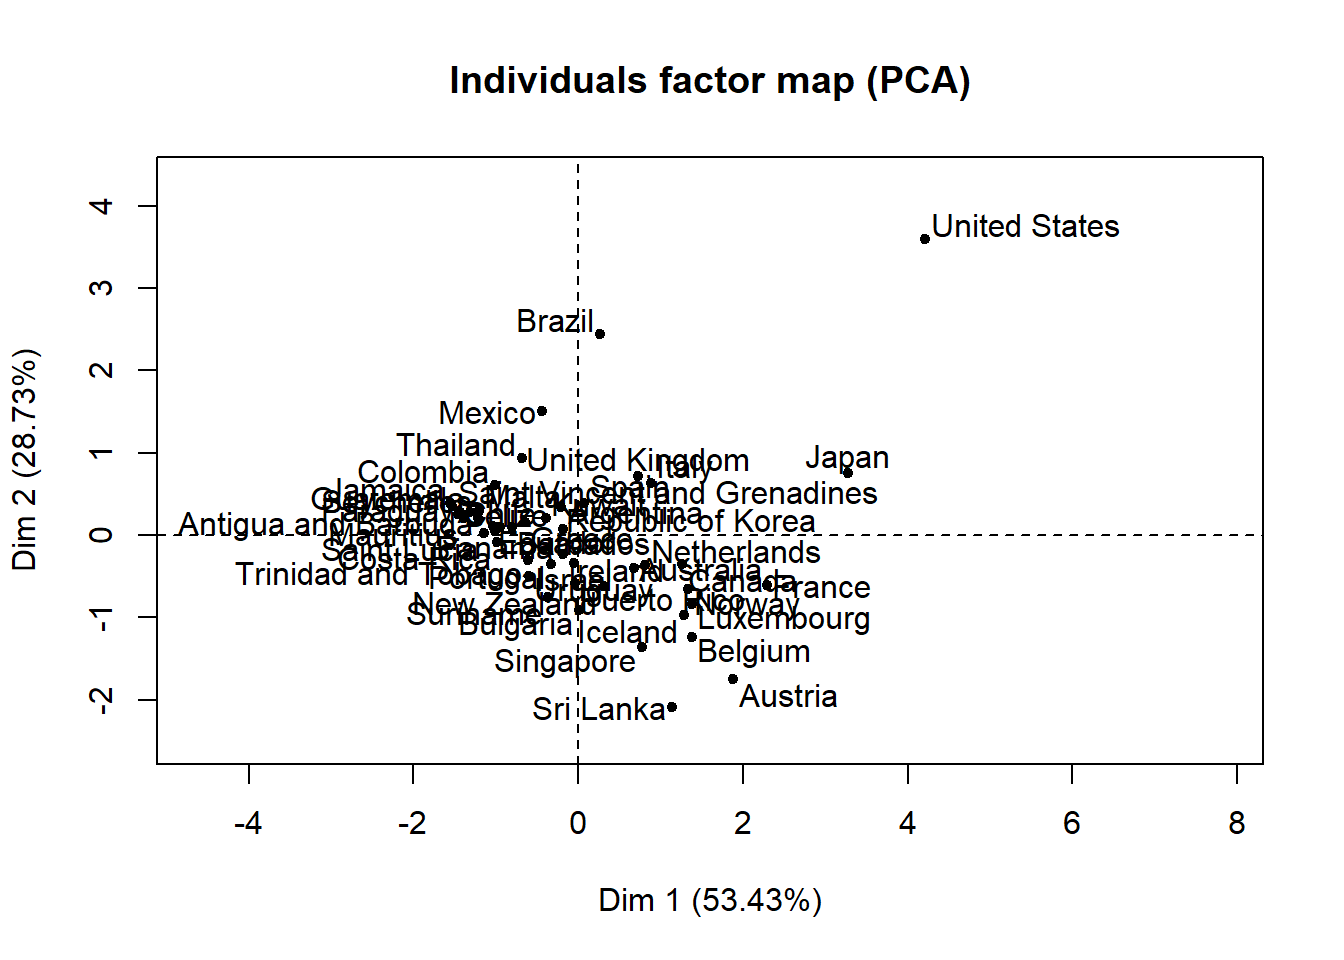
\includegraphics{football-cluster_files/figure-latex/unnamed-chunk-33-1.pdf}

\begin{Shaded}
\begin{Highlighting}[]
\KeywordTok{fviz_pca_ind}\NormalTok{(pca, }\DataTypeTok{geom =} \StringTok{"point"}\NormalTok{, }
             \DataTypeTok{alpha.ind =} \StringTok{"contrib"}\NormalTok{, }\DataTypeTok{addEllipses =}\NormalTok{ T) }\OperatorTok{+}\StringTok{ }\KeywordTok{theme_economist}\NormalTok{() }\OperatorTok{+}
\StringTok{  }\KeywordTok{xlim}\NormalTok{(}\KeywordTok{c}\NormalTok{(}\OperatorTok{-}\DecValTok{6}\NormalTok{, }\DecValTok{-10}\NormalTok{))}
\end{Highlighting}
\end{Shaded}

\begin{verbatim}
## Warning: Removed 16778 rows containing non-finite values (stat_ellipse).
\end{verbatim}

\begin{verbatim}
## Warning: Removed 16778 rows containing missing values (geom_point).
\end{verbatim}

\begin{verbatim}
## Warning: Removed 1 rows containing missing values (geom_vline).
\end{verbatim}

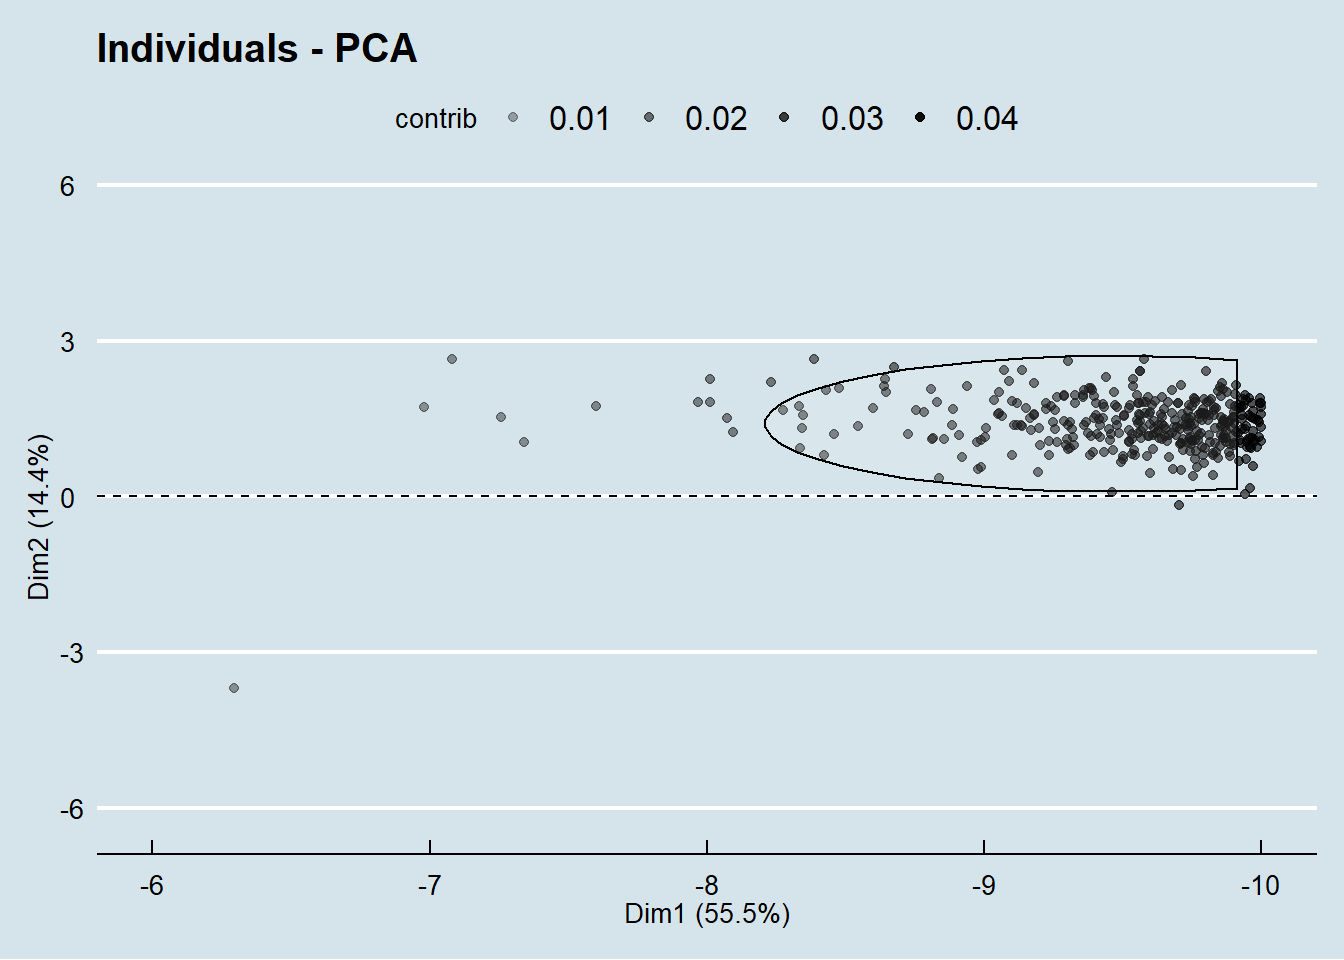
\includegraphics{football-cluster_files/figure-latex/unnamed-chunk-34-1.pdf}

\begin{Shaded}
\begin{Highlighting}[]
\KeywordTok{fviz_pca_ind}\NormalTok{(pca, }\DataTypeTok{geom =} \StringTok{"text"}\NormalTok{, }
             \DataTypeTok{select.ind =} \KeywordTok{list}\NormalTok{(}\DataTypeTok{name =} \KeywordTok{c}\NormalTok{(}\StringTok{"L. Messi"}\NormalTok{, }
                                        \StringTok{"Cristiano Ronaldo"}\NormalTok{, }\StringTok{"Neymar Jr"}\NormalTok{, }\StringTok{"E. Hazard"}\NormalTok{))) }\OperatorTok{+}\StringTok{ }
\StringTok{  }\KeywordTok{theme_economist}\NormalTok{()}
\end{Highlighting}
\end{Shaded}

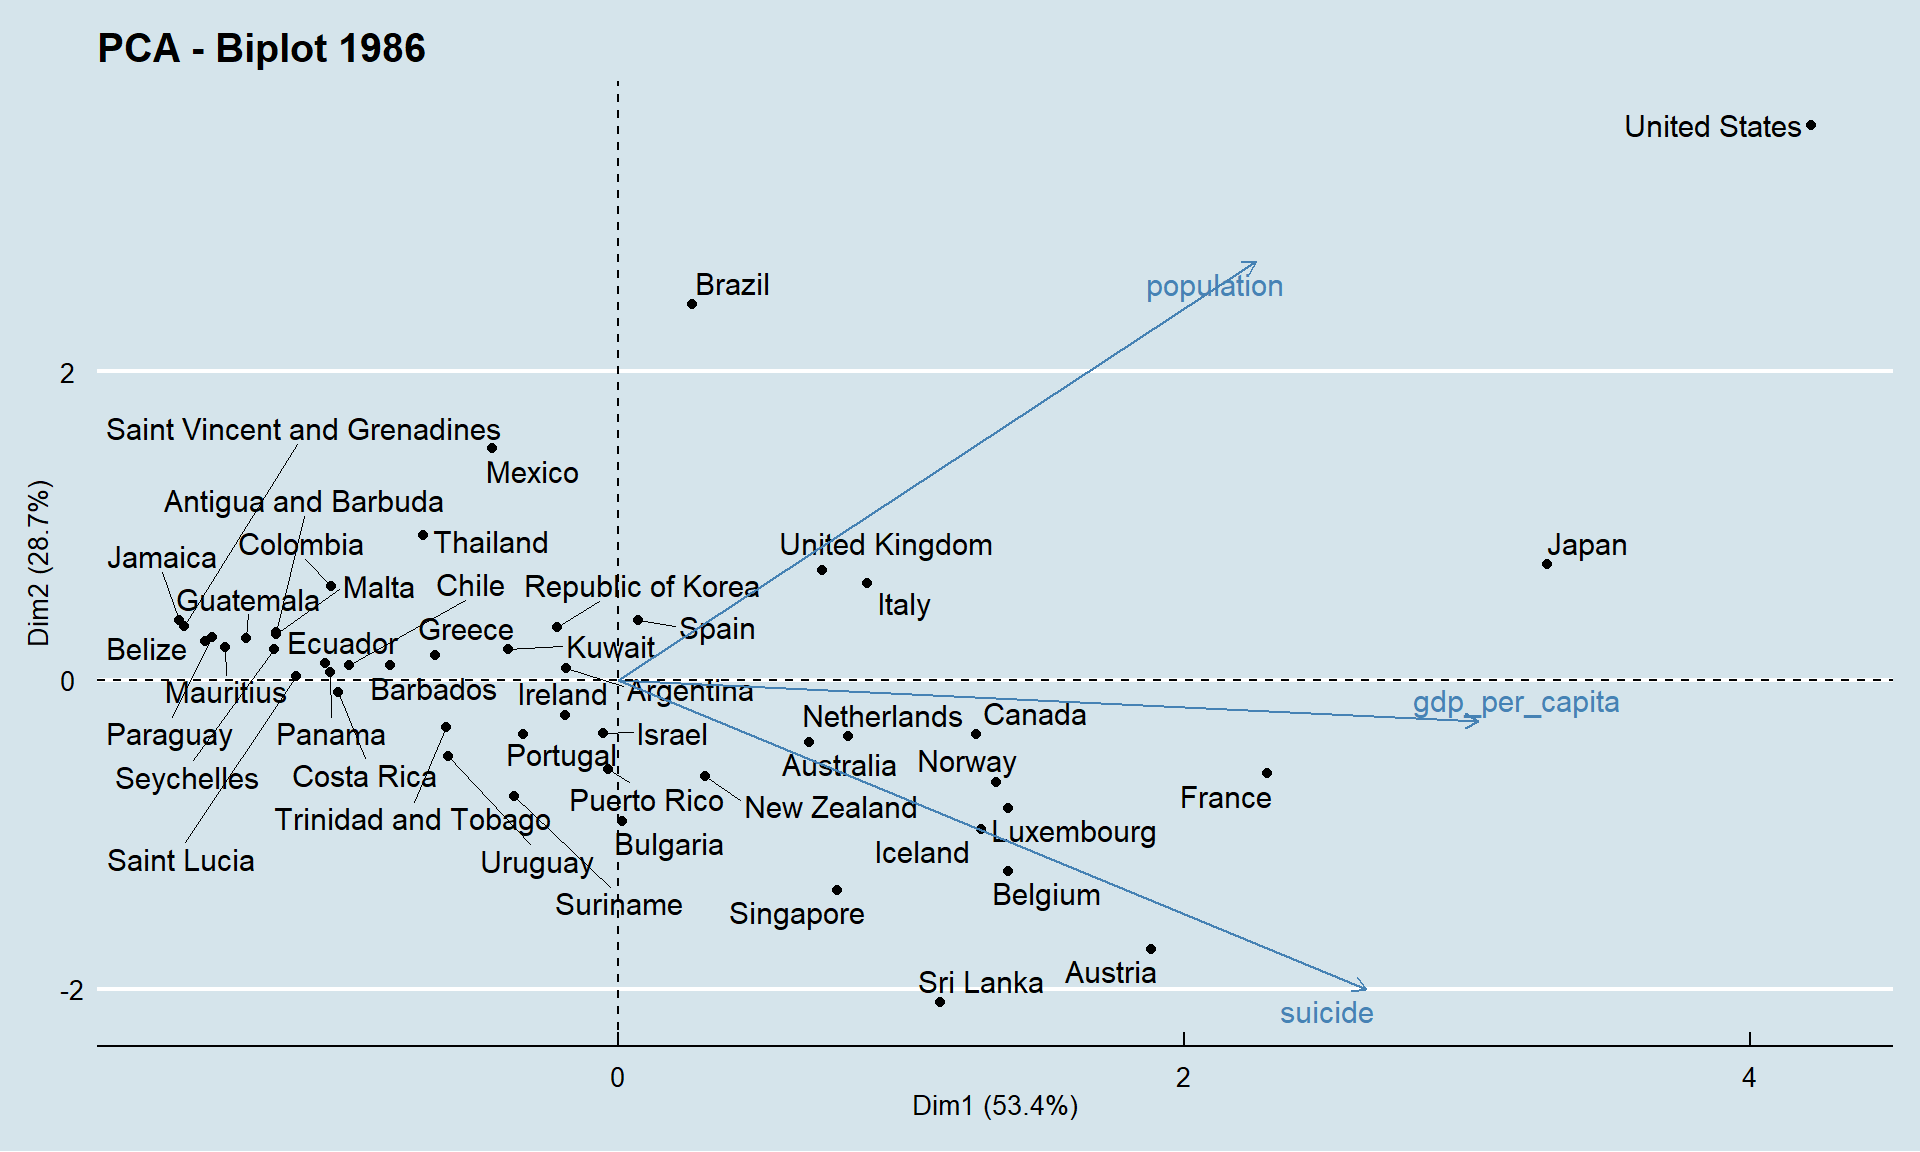
\includegraphics{football-cluster_files/figure-latex/unnamed-chunk-35-1.pdf}


\end{document}
